\documentclass[xcolor=pdflatex,dvipsnames,table]{beamer}
\usepackage{epsfig,graphicx}
\usepackage{palatino}
\usepackage{fancybox}
\usepackage{relsize}
\usepackage[procnames]{listings}

% "define" Scala
\usepackage[T1]{fontenc}  
\usepackage[scaled=0.82]{beramono}  
\usepackage{microtype} 

\sbox0{\small\ttfamily A}
\edef\mybasewidth{\the\wd0 }

\lstdefinelanguage{scala}{
  morekeywords={abstract,case,catch,class,def,%
    do,else,extends,false,final,finally,%
    for,if,implicit,import,match,mixin,%
    new,null,object,override,package,%
    private,protected,requires,return,sealed,%
    super,this,throw,trait,true,try,%
    type,val,var,while,with,yield},
  sensitive=true,
  morecomment=[l]{//},
  morecomment=[n]{/*}{*/},
  morestring=[b]",
  morestring=[b]',
  morestring=[b]"""
}

\usepackage{color}
\definecolor{dkgreen}{rgb}{0,0.6,0}
\definecolor{gray}{rgb}{0.5,0.5,0.5}
\definecolor{mauve}{rgb}{0.58,0,0.82}

% Default settings for code listings
\lstset{language=scala,
  showstringspaces=false,
  columns=fixed, % basewidth=\mybasewidth,
  basicstyle={\small\ttfamily},
  numbers=none,
  numberstyle=\footnotesize\color{gray},
  % identifierstyle=\color{red},
  keywordstyle=\color{blue},
  commentstyle=\color{dkgreen},
  stringstyle=\color{mauve},
  breakatwhitespace=true,
  procnamekeys={def, val, var, class, trait, object, extends},
  procnamestyle=\ttfamily\color{red},
}

\lstnewenvironment{scala}
{\lstset{language=scala}}
{}
\lstnewenvironment{cpp}
{\lstset{language=C++}}
{}
\lstnewenvironment{bash}
{\lstset{language=bash}}
{}
\lstnewenvironment{verilog}
{\lstset{language=verilog}}
{}

\newcommand{\isc}{
\lstinline
}

\lstdefinestyle{scala}{language=scala,
  showstringspaces=false,
  columns=fixed, % basewidth=\mybasewidth,
  basicstyle={\small\ttfamily},
  numbers=none,
  numberstyle=\footnotesize\color{gray},
  % identifierstyle=\color{red},
  keywordstyle=\color{blue},
  commentstyle=\color{dkgreen},
  stringstyle=\color{mauve},
  breakatwhitespace=true,
  procnamekeys={def, val, var, class, trait, object, extends},
  procnamestyle=\ttfamily\color{red},
}

\lstset{basicstyle={\footnotesize\ttfamily}}

\usetheme[height=8mm]{Rochester}
\setbeamersize{text margin left=3mm} 
\setbeamersize{text margin right=3mm} 
\setbeamertemplate{navigation symbols}{}

\definecolor{Cobalt}{rgb}{0.25,0.125,0.70}
\definecolor{RedOrange}{rgb}{0.8,0.25,0.0}
% \definecolor{RedOrange}{rgb}{0.8,0.775,0.25}
\def\frametitledefaultcolor{Cobalt}
\def\frametitleproblemcolor{RedOrange}

\lstset{basicstyle={\footnotesize\ttfamily}}

\setbeamertemplate{frametitle}
{
\vskip-7mm
\textbf{\insertframetitle}\hfill\insertframenumber
}
\setbeamercolor{frametitle}{bg=\frametitledefaultcolor}

\newenvironment{sample}{\VerbatimEnvironment\begin{footnotesize}\begin{semiverbatim}}{\end{semiverbatim}\end{footnotesize}}

\newenvironment{FramedSemiVerb}%
{\begin{Sbox}\begin{minipage}{.94\textwidth}\begin{semiverbatim}}%
{\end{semiverbatim}\end{minipage}\end{Sbox}
\setlength{\fboxsep}{8pt}\fbox{\TheSbox}}

\newenvironment{FramedVerb}%
{\VerbatimEnvironment
\begin{Sbox}\begin{minipage}{.94\textwidth}\begin{Verbatim}}%
{\end{Verbatim}\end{minipage}\end{Sbox}
\setlength{\fboxsep}{8pt}\fbox{\TheSbox}}

% \newenvironment{sample}{\VerbatimEnvironment\begin{footnotesize}\begin{Verbatim}}{\end{Verbatim}\end{footnotesize}}
\newcommand{\code}[1]{\begin{footnotesize}{\tt #1}\end{footnotesize}}
\newcommand{\comment}[1]{{\color{Green}\it\smaller #1}}


\title{Chisel Bootcamp}
\author{Jonathan Bachrach}
\date{\today}
\institute[UC Berkeley]{EECS UC Berkeley}

\begin{document}

\begin{frame}
\titlepage
\end{frame}
\addtocounter{framenumber}{-1}

% \begin{frame}[fragile]{tutorial.scala}
% \begin{scala}
% package Tutorial {
% 
% import Chisel._
% 
% object Tutorial {
%   def main(args: Array[String]): Unit = { 
%     val tut_args = args.slice(1, args.length) ++ 
%       Array("--targetDir", "../emulator", "--genHarness")
%     args(0) match {
%       case "gcd" => 
%         chiselMain(tut_args, () => new GCD())
%       ...
%     }
%   }
% }
% 
% }
% \end{scala}
% \end{frame}

\begin{frame}[fragile]{Goals for Bootcamp}

\begin{itemize}
\item get you started with Chisel
\item get a basic working knowledge of Chisel
\item learn how to think in Chisel
\item know where to get more information
\end{itemize}

\end{frame}

\setbeamercolor{frametitle}{bg=\frametitleproblemcolor}
\begin{frame}[fragile]{Bootcamp Chisel Installation}
\begin{scala}
-Install VirtualBox
-File->Import appliance, chisel-vm.ova
-Start
-Login (username: chisel-bootcamp, password: chisel)
-GTKWave, Emacs, etc. all installed
\end{scala}
\end{frame}
\setbeamercolor{frametitle}{bg=\frametitledefaultcolor}

\setbeamercolor{frametitle}{bg=\frametitleproblemcolor}
\begin{frame}[fragile]{Development Tool Installation}

\begin{itemize}
\item {\bf MacOSX}:

\begin{itemize}
\item Install XCODE, including console tools.
\end{itemize}

\item {\bf Linux}: 

\begin{itemize}
\item To prepare your Linux platform for Chisel, you will need to install the following packages:
\begin{itemize}
\item \verb|g++| 
\item \verb+openjdk-7-jre+
\end{itemize}
\item using 
\begin{itemize}
\item \verb+sudo apt-get install+
\end{itemize}
\end{itemize}

\end{itemize}
\end{frame}
\setbeamercolor{frametitle}{bg=\frametitledefaultcolor}

\setbeamercolor{frametitle}{bg=\frametitleproblemcolor}
\begin{frame}[fragile]{Getting the Chisel Tutorial}

\begin{scala}
git clone https://github.com/ucb-bar/chisel-tutorial.git
cd chisel-tutorial
\end{scala}
\end{frame}
\setbeamercolor{frametitle}{bg=\frametitledefaultcolor}

\setbeamercolor{frametitle}{bg=\frametitleproblemcolor}
\begin{frame}[fragile]{Chisel Tutorial Contents}
\begin{FramedSemiVerb}
chisel-tutorial/  
  Makefile
  examples/   \comment{\# Contains chisel examples}
    Makefile  
    build.sbt \comment{\# Contains project description}
    FullAdder.scala ...
  problems/   \comment{\# Contains skeletal files for tutorial problems}
    Makefile
    build.sbt \comment{\# Contains project description}
    Accumulator.scala ...
  solutions/  \comment{\# Contains solutions to problems}
    Makefile
    build.sbt \comment{\# Contains project description}
    Counter.scala ...
\end{FramedSemiVerb}
\end{frame}
\setbeamercolor{frametitle}{bg=\frametitledefaultcolor}

\setbeamercolor{frametitle}{bg=\frametitleproblemcolor}
\begin{frame}[fragile]{Test It}

\begin{bash}
cd $TUT_DIR
make 
\end{bash}

% \begin{bash}
% cd $TUT_DIR/examples
% make check Parity.out
% \end{bash}

\vspace{1cm}
\noindent
If your system is set up correctly, you should see a messsage \verb+[success]+ followed by the total time of the run, and date and time of completion. 

\end{frame}
\setbeamercolor{frametitle}{bg=\frametitledefaultcolor}


\setbeamercolor{frametitle}{bg=\frametitleproblemcolor}
\begin{frame}[fragile]{Get This}

\begin{center}
\fbox{
\url{chisel.eecs.berkeley.edu/chisel-bootcamp.pdf}
}
\end{center}

\end{frame}
\setbeamercolor{frametitle}{bg=\frametitledefaultcolor}

\begin{frame}[fragile]
\frametitle{Chisel}

\begin{columns}[c]

\column{0.55\textwidth}

\begin{itemize}
\item A hardware construction language 
\begin{itemize}
\item ``synthesizable by construction''
\item creates graph representing hardware
\end{itemize}
\item Embedded within Scala language to leverage mindshare and language design
\item Best of hardware and software design ideas
\item Multiple targets
\begin{itemize}
\item Simulation and synthesis
\item Memory IP is target-specific \\[0.5cm]
\end{itemize}
\item {\color{red}{\bf Not} Scala app -> Verilog arch}
\end{itemize}

\column{0.40\textwidth}

\begin{center}
single source \\
\includegraphics[width=0.99\textwidth]{../talks/retreat-1/figs/graph-and-targets.pdf} \\
multiple targets \\
\end{center}

\end{columns}
\note{creates a graph if successfully created will correctly synthesize \\[1cm]
single source generates two different verilog outputs, one for fpga and one for asic. \\[1cm]
surprisingly difficult to generate each.  for example, chisel has abstraction for memories.}
\end{frame}

\begin{frame}[fragile]
\frametitle{The Scala Programming Language}

\begin{columns}[c]

\column{0.75\textwidth}

\begin{itemize}
\item Object Oriented
\begin{itemize}
\item Factory Objects, Classes
\item Traits, overloading etc
\item Strongly typed with type inference
\end{itemize}
\item Functional
\begin{itemize}
\item Higher order functions
\item Anonymous functions
\item Currying etc
\end{itemize}
\item Extensible
\begin{itemize}
\item Domain Specific Languages (DSLs)
\end{itemize}
\item Compiled to JVM
\begin{itemize}
\item Good performance
\item Great Java interoperability
\item Mature debugging, execution environments
\end{itemize}
\item Growing Popularity
\begin{itemize}
\item Twitter
\item many Universities
\end{itemize}
\end{itemize}

\column{0.25\textwidth}

\begin{center}

\includegraphics[height=0.4\textheight]{figs/programming-scala.pdf} \\
\includegraphics[height=0.4\textheight]{figs/programming-in-scala.pdf}
\end{center}

\end{columns}
\note{powerful combination of scipting and type safety, \\[1cm]
includes powerful features to support abstraction, \\[1cm]
as makes it easy to embed DSLs, compiles to jvm}
\end{frame}

\begin{frame}[fragile]{Scala Bindings}
\begin{scala}
// constant
val x = 1
val (x, y) = (1, 2)

// variable
var y = 2
y = 3
\end{scala}
\end{frame}

\begin{frame}[fragile]{Scala Collections}
\begin{scala}
// Array's
val tbl = new Array[Int](256)
tbl(0) = 32
val y = tbl(0)
val n = tbl.length

// ArrayBuffer's
import scala.collection.mutable.ArrayBuffer
val buf = new ArrayBuffer[Int]()
buf += 12
val z = buf(0)
val l = buf.length

// List's
val els = List(1, 2, 3)
val els2 = x :: y :: y :: Nil
val a :: b :: c :: Nil = els
val m = els.length

\end{scala}
\end{frame}

% // Tuple's
% val (x, y, z) = (1, 2, 3)


\begin{frame}[fragile]{Scala Iteration}
\begin{scala}
val tbl = new Array[Int](256)

// loop over all indices
for (i <- 0 until tbl.length)
  tbl(i) = i

// loop of each sequence element
val tbl2 = new ArrayBuffer[Int]
for (e <- tbl)
  tbl2 += 2*e
\end{scala}

% // create second table with doubled elements
% val tbl2 = for (i <- 0 until 16) yield tbl(i)*2
% // nested loop
% for (i <- 0 until 16; j <- 0 until 16)
%   tbl(j*16 + i) = i

\end{frame}

\begin{frame}[fragile]{Scala Functions}
\begin{scala}
// simple scaling function, e.g., x2(3) => 6
def x2 (x: Int) = 2 * x
\end{scala}

\begin{scala}
// more complicated function with statements
def f (x: Int, y: Int) = {
  val xy = x + y;
  if (x < y) xy else -xy
}
\end{scala}
\end{frame}

\begin{frame}[fragile]{Scala Functional}
\begin{scala}
// simple scaling function, e.g., x2(3) => 6
def x2 (x: Int) = 2 * x
\end{scala}

\begin{scala}
// produce list of 2 * elements, e.g., x2list(List(1, 2, 3)) => List(2, 4, 6)
def x2list (xs: List[Int]) = xs.map(x2)
\end{scala}

\begin{scala}
// simple addition function, e.g., add(1, 2) => 3
def add (x: Int, y: Int) = x + y
\end{scala}

\begin{scala}
// sum all elements using pairwise reduction, e.g., sum(List(1, 2, 3)) => 6
def sum (xs: List[Int]) = xs.foldLeft(0)(add)
\end{scala}
\end{frame}

\begin{frame}[fragile]{Scala Object Oriented}

\begin{scala}
class Blimp(r: Double) {
  val rad = r
  println("Another Blimp")
}

new Blimp(10.0)
\end{scala}

\begin{scala}
class Zep(h: Boolean, r: Double) extends Blimp(r) {
  val isHydrogen = h
}

new Zep(true, 100.0)
\end{scala}

\end{frame}

\begin{frame}[fragile]{Scala Singleton Objects}

\begin{itemize}
\item like Java class methods
\item for top level methods
\end{itemize}
\begin{scala}
object Blimp {
  var numBlimps = 0
  def apply(r: Double) = {
    numBlimps += 1
    new Blimp(r)
  }
}

Blimp.numBlimps
Blimp(10.0)
\end{scala}

\end{frame}

% \begin{frame}[fragile]{Cloning}
% \begin{itemize}
% \item shallow copy of object
% \item user can override method to incorporate parameters
% \item \verb+this.type+ allows precise return types
% \end{itemize}
% \begin{scala}
% class Blimp(r: Double) {
%   val rad = r
%   override def clone(): this.type = new Blimp(r)
% }
% 
% val b1 = new Blimp(10)
% val b2 = b1.clone()
% \end{scala}
% \end{frame}
% \begin{frame}[fragile]{Scala Console}
% \begin{scala}
% > scala
% scala> 1 + 2
% => 3
% scala> def f (x: Int) = 2 * x
% => (Int) => Int
% scala> f(4)
% => 8
% \end{scala}
% \end{frame}
% 


\begin{frame}[fragile]
\frametitle{Algebraic Graph Construction}

\begin{columns}
\column{0.35\textwidth}
{\lstset{basicstyle={\Large\ttfamily}}
\begin{scala}
Mux(x > y, x, y)
\end{scala}
}

\column{0.6\textwidth}

\begin{center}
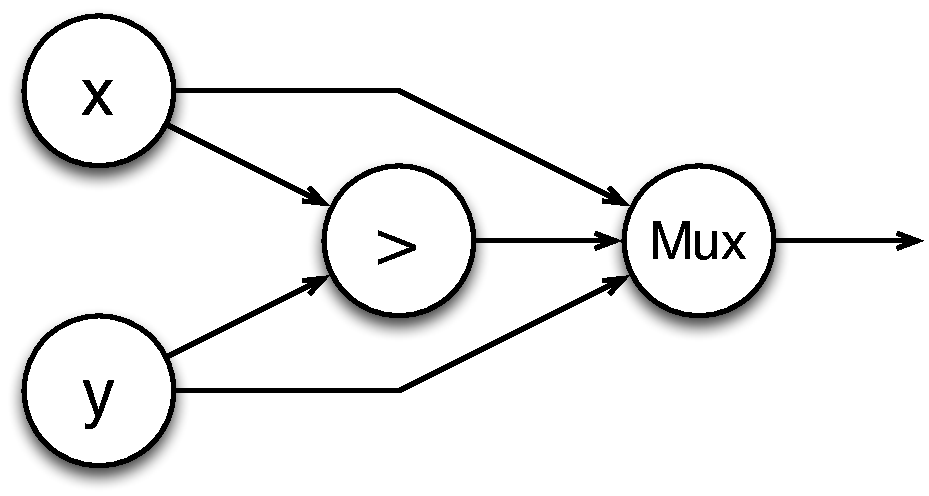
\includegraphics[width=0.9\textwidth]{figs/max2.pdf} 
\end{center}
\end{columns}
\end{frame}

\begin{frame}[fragile]
\frametitle{Creating Module}

\begin{columns}
\column{0.45\textwidth}

{\lstset{basicstyle={\scriptsize\ttfamily}}
\begin{scala}
class Max2 extends Module {
  val io = new Bundle {
    val x = UInt(INPUT, 8)
    val y = UInt(INPUT, 8)
    val z = UInt(OUTPUT, 8) }
  io.z := Mux(io.x > io.y, io.x, io.y)
}
\end{scala}
}

\column{0.45\textwidth}
\begin{center}
\includegraphics[width=0.95\textwidth]{figs/Max2c.pdf} \\
\end{center}
\end{columns}

\end{frame}

\begin{frame}[fragile]
\frametitle{Connecting Modules}

\begin{columns}
\column{0.3\textwidth}
\begin{scala}
val m1 = 
  Module(new Max2())
m1.io.x := a
m1.io.y := b
val m2 = 
  Module(new Max2())
m2.io.x := c
m2.io.y := d
val m3 = 
  Module(new Max2())
m3.io.x := m1.io.z
m3.io.y := m2.io.z
\end{scala}

\column{0.6\textwidth}

\begin{center}
\includegraphics[width=0.99\textwidth]{figs/Max4.pdf} \\
\end{center}
\end{columns}

\end{frame}


\begin{frame}[fragile]
\frametitle{Defining Construction Functions}

\begin{columns}

\column{0.45\textwidth}

\begin{scala}
def Max2(x, y) = Mux(x > y, x, y)
\end{scala}
\begin{scala}
Max2(x, y)
\end{scala}

\column{0.5\textwidth}

\begin{center}
\includegraphics[width=0.95\textwidth]{figs/Max2.pdf} \\[1cm]
\end{center}

\end{columns}

\end{frame}

\begin{frame}[fragile]
\frametitle{Functional Construction}

\begin{columns}

\column{0.5\textwidth}

{\lstset{basicstyle={\scriptsize\ttfamily}}
\begin{scala}
class MaxN(n: Int, w: Int) extends Module {
  val io = new Bundle {
    val in  = Vec.fill(n){ UInt(INPUT, w) }
    val out = UInt(OUTPUT, w)
  }
  io.out := io.in.reduceLeft(Max2)
}
\end{scala}
}

\column{0.4\textwidth}

\begin{center}
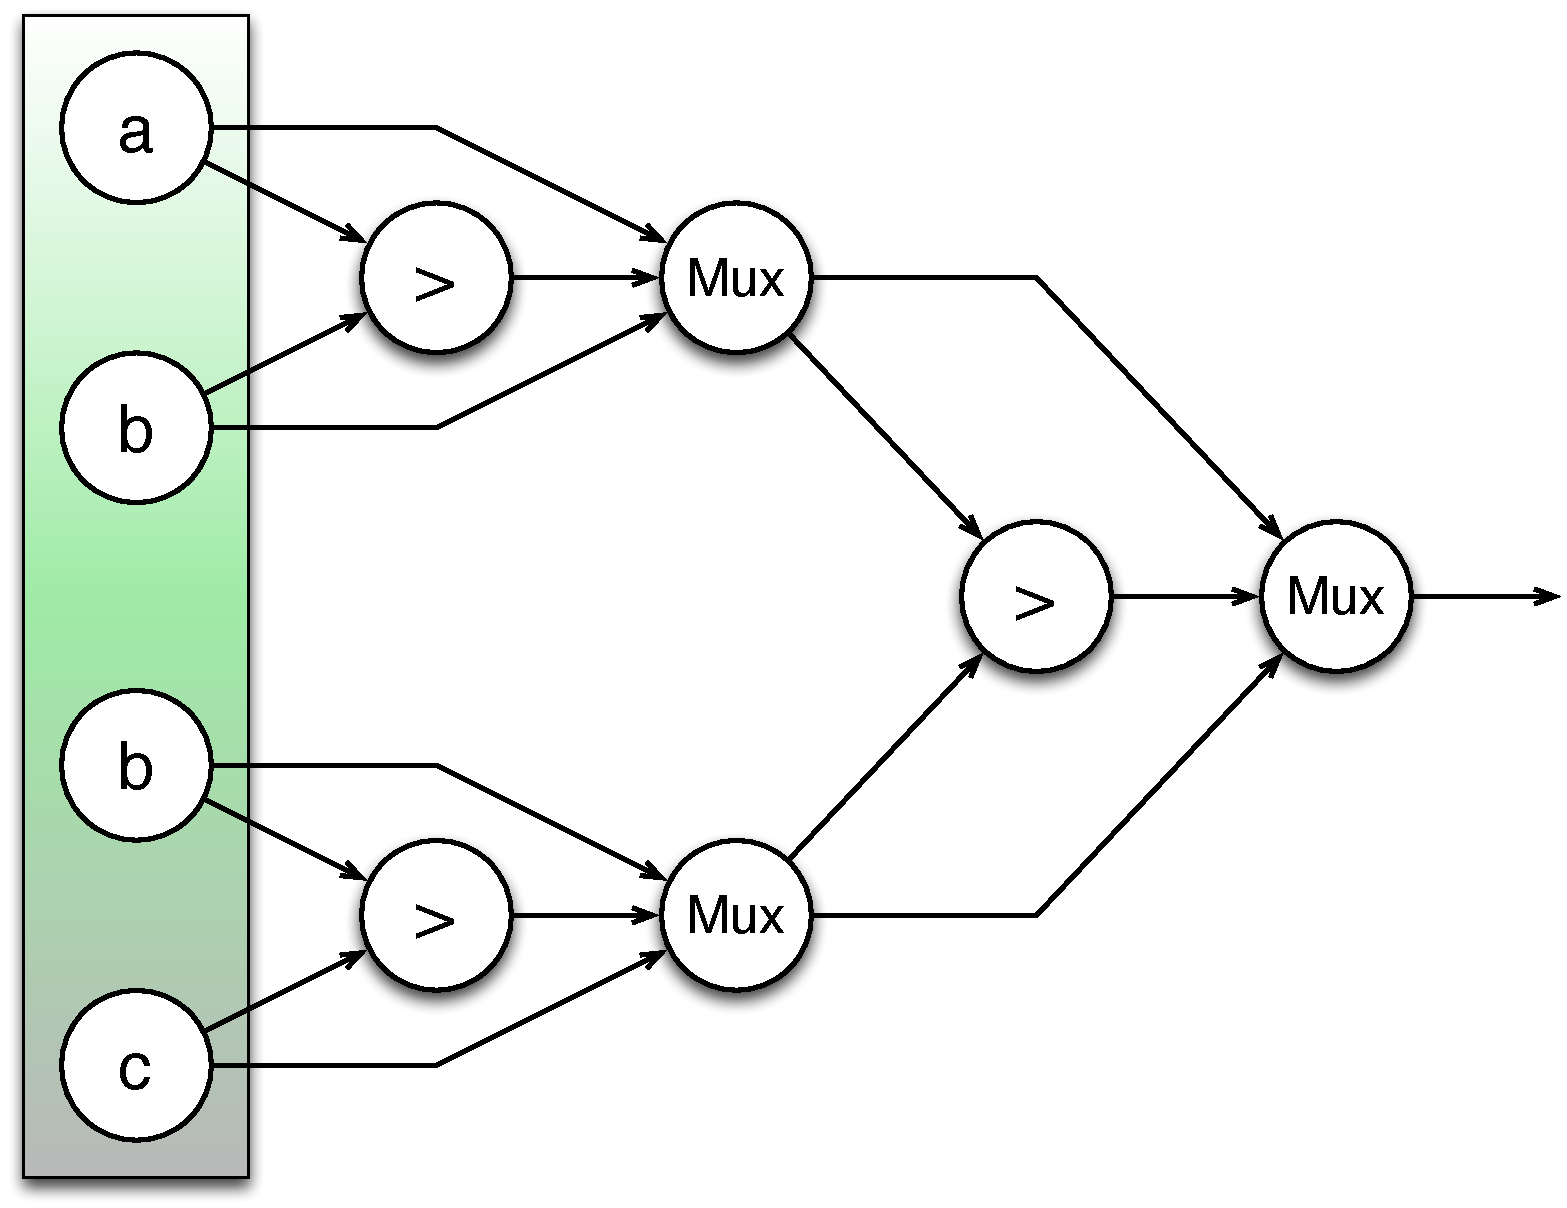
\includegraphics[width=0.99\textwidth]{figs/reduceMax.pdf} \\
\end{center}

\end{columns}

\end{frame}

\begin{frame}[fragile]
\frametitle{Example}
\begin{columns}

\column{0.45\textwidth}

\begin{footnotesize}
\begin{scala}
class GCD extends Module {
  val io = new Bundle {
    val a     = UInt(INPUT, 16)
    val b     = UInt(INPUT, 16)
    val z     = UInt(OUTPUT, 16)
    val valid = Bool(OUTPUT) }
  val x = Reg(init = io.a)
  val y = Reg(init = io.b)
  when (x > y) {
    x := x - y
  } .otherwise {
    y := y - x
  }
  io.z     := x
  io.valid := y === UInt(0)
}
\end{scala}
\end{footnotesize}

\column{0.45\textwidth}

\begin{center}
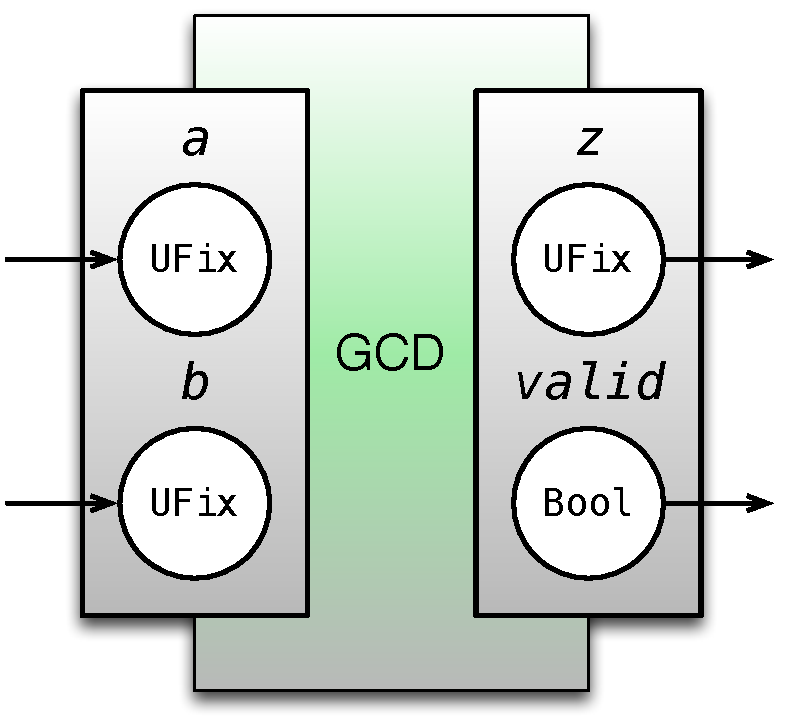
\includegraphics[width=0.9\textwidth]{figs/gcd.pdf} 
\end{center}

\end{columns}
\end{frame}

\setbeamercolor{frametitle}{bg=\frametitleproblemcolor}
\begin{frame}[fragile]{Running the Chisel Simulation}

\begin{bash}
cd ~/chisel-tutorial/examples
make GCD.out
\end{bash}

{\lstset{basicstyle={\scriptsize\ttfamily}}
\begin{bash}
...
PASSED
[success] Total time: 2 s, completed Feb 28, 2013 8:14:37 PM
\end{bash}
}

\end{frame}
\setbeamercolor{frametitle}{bg=\frametitledefaultcolor}

\setbeamercolor{frametitle}{bg=\frametitleproblemcolor}
\begin{frame}[fragile]{Generating Verilog}

\begin{bash}
cd ~/chisel-tutorial/examples
make GCD.v
\end{bash}

The Verilog source is roughly divided into three parts:

\begin{enumerate}
\item Module declaration with input and outputs
\item Temporary wire and register declaration used for holding intermediate values
\item Register assignments in \verb+always @ (posedge clk)+
\end{enumerate}

\end{frame}
\setbeamercolor{frametitle}{bg=\frametitledefaultcolor}

\begin{frame}[fragile]{FullAdder -- Type Inference}

\begin{columns}
\column{0.4\textwidth}

{\lstset{basicstyle={\scriptsize\ttfamily}}
\begin{scala}
class FullAdder extends Module {
  val io = new Bundle {
    val a    = UInt(INPUT, 1)
    val b    = UInt(INPUT, 1)
    val cin  = UInt(INPUT, 1)
    val sum  = UInt(OUTPUT, 1)
    val cout = UInt(OUTPUT, 1)
  }
  // Generate the sum
  val a_xor_b = io.a ^ io.b
  io.sum := a_xor_b ^ io.cin
  // Generate the carry
  val a_and_b   = io.a & io.b
  val b_and_cin = io.b & io.cin
  val a_and_cin = io.a & io.cin
  io.cout := 
    a_and_b | b_and_cin | a_and_cin
}
\end{scala}
}

\column{0.55\textwidth}

\begin{center}
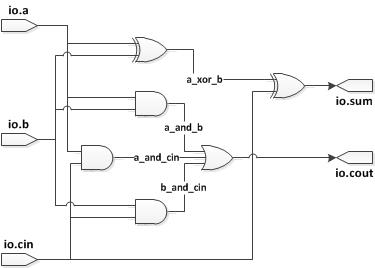
\includegraphics[width=0.9\textwidth]{../getting-started/figs/Full_Adder.jpg}
\end{center}

\end{columns}

\end{frame}

\begin{frame}[fragile]{FullAdder Verilog -- Width Inference 1}

\begin{columns}
\column{0.45\textwidth}

{\lstset{basicstyle={\scriptsize\ttfamily}}
\begin{scala}
class FullAdder extends Module {
  val io = new Bundle {
    val a    = UInt(INPUT, 1)
    val b    = UInt(INPUT, 1)
    val cin  = UInt(INPUT, 1)
    val sum  = UInt(OUTPUT, 1)
    val cout = UInt(OUTPUT, 1)
  }
  // Generate the sum
  val a_xor_b = io.a ^ io.b
  io.sum := a_xor_b ^ io.cin
  // Generate the carry
  val a_and_b   = io.a & io.b
  val b_and_cin = io.b & io.cin
  val a_and_cin = io.a & io.cin
  io.cout := 
    a_and_b | b_and_cin | a_and_cin
}
\end{scala}
}

\column{0.45\textwidth}

{\lstset{basicstyle={\scriptsize\ttfamily}}
\begin{scala}
module FullAdder(
    input  io_a,
    input  io_b,
    input  io_cin,
    output io_sum,
    output io_cout);
  wire T0;
  wire a_and_cin;
  wire T1;
  wire b_and_cin;
  wire a_and_b;
  wire T2;
  wire a_xor_b;

  assign io_cout = T0;
  assign T0 = T1 | a_and_cin;
  assign a_and_cin = io_a & io_cin;
  assign T1 = a_and_b | b_and_cin;
  assign b_and_cin = io_b & io_cin;
  assign a_and_b = io_a & io_b;
  assign io_sum = T2;
  assign T2 = a_xor_b ^ io_cin;
  assign a_xor_b = io_a ^ io_b;
endmodule
\end{scala}
}

\end{columns}

\end{frame}

\begin{frame}[fragile]{FullAdder2 Verilog -- Width Inference 2}

\begin{columns}
\column{0.45\textwidth}

{\lstset{basicstyle={\scriptsize\ttfamily}}
\begin{scala}
class FullAdder2 extends Module {
  val io = new Bundle {
    val a    = UInt(INPUT, 2)
    val b    = UInt(INPUT, 2)
    val cin  = UInt(INPUT, 2)
    val sum  = UInt(OUTPUT, 2)
    val cout = UInt(OUTPUT, 2)
  }
  // Generate the sum
  val a_xor_b = io.a ^ io.b
  io.sum := a_xor_b ^ io.cin
  // Generate the carry
  val a_and_b   = io.a & io.b
  val b_and_cin = io.b & io.cin
  val a_and_cin = io.a & io.cin
  io.cout := 
    a_and_b | b_and_cin | a_and_cin
}
\end{scala}
}

\column{0.45\textwidth}

{\lstset{basicstyle={\scriptsize\ttfamily}}
\begin{scala}
module FullAdder(
    input [1:0] io_a,
    input [1:0] io_b,
    input [1:0] io_cin,
    output[1:0] io_sum,
    output[1:0] io_cout);
  wire[1:0] T0;
  wire[1:0] a_and_cin;
  wire[1:0] T1;
  wire[1:0] b_and_cin;
  wire[1:0] a_and_b;
  wire[1:0] T2;
  wire[1:0] a_xor_b;

  assign io_cout = T0;
  assign T0 = T1 | a_and_cin;
  assign a_and_cin = io_a & io_cin;
  assign T1 = a_and_b | b_and_cin;
  assign b_and_cin = io_b & io_cin;
  assign a_and_b = io_a & io_b;
  assign io_sum = T2;
  assign T2 = a_xor_b ^ io_cin;
  assign a_xor_b = io_a ^ io_b;
endmodule
\end{scala}
}

\end{columns}

\end{frame}

\begin{frame}[fragile]{Using Registers}
\begin{scala}
// clock the new reg value on every cycle
val y = io.x
val z = Reg(next = y)
\end{scala}

\begin{scala}
// clock the new reg value when the condition a > b
val x = Reg(UInt())
when (a > b) { x := y }
.elsewhen (b > a) { x := z }
.otherwise { x := w }
\end{scala}
\end{frame}

\begin{frame}[fragile]{Unconditional Register Update}

\begin{columns}

\column{0.42\textwidth}

{\lstset{basicstyle={\scriptsize\ttfamily}}
\begin{scala}
class ShiftRegister extends Module {
  val io = new Bundle {
    val in  = UInt(INPUT, 1)
    val out = UInt(OUTPUT, 1)
  }
  val r0 = Reg(next = io.in)
  val r1 = Reg(next = r0)
  val r2 = Reg(next = r1)
  val r3 = Reg(next = r2)
  io.out := r3
}
\end{scala}
}
\begin{center}
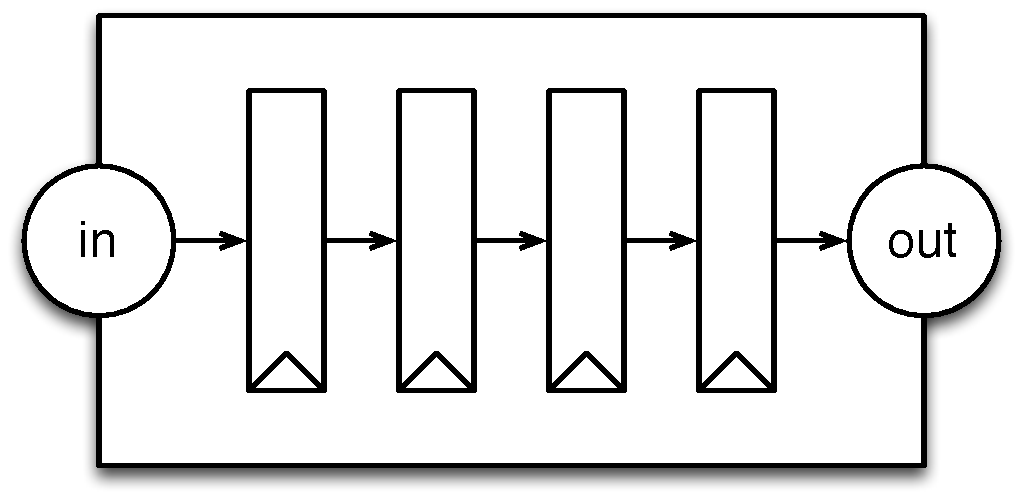
\includegraphics[width=0.9\textwidth]{figs/shift-register.pdf}
\end{center}

\column{0.5\textwidth}

{\lstset{basicstyle={\scriptsize\ttfamily}}
\begin{scala}
module ShiftRegister(input clk, input reset,
    input  io_in,
    output io_out);

  reg[0:0] r3;
  reg[0:0] r2;
  reg[0:0] r1;
  reg[0:0] r0;

  assign io_out = r3;
  always @(posedge clk) begin
    r3 <= r2;
    r2 <= r1;
    r1 <= r0;
    r0 <= io_in;
  end
endmodule
\end{scala}
}

\end{columns}

\end{frame}

\begin{frame}[fragile]{Conditional Register Update}

\begin{columns}

\column{0.47\textwidth}

\begin{scala}
class ShiftRegister extends Module {
  val io = new Bundle {
    val in    = UInt(INPUT, 1)
    val shift = Bool(INPUT)
    val out   = UInt(OUTPUT, 1)
  }

  val r0 = Reg(UInt())
  val r1 = Reg(UInt())
  val r2 = Reg(UInt())
  val r3 = Reg(UInt())

  when (io.shift) {
    r0 := io.in
    r1 := r0
    r2 := r1
    r3 := r2
  }
  io.out := r3
}
\end{scala}

\column{0.45\textwidth}

\begin{center}
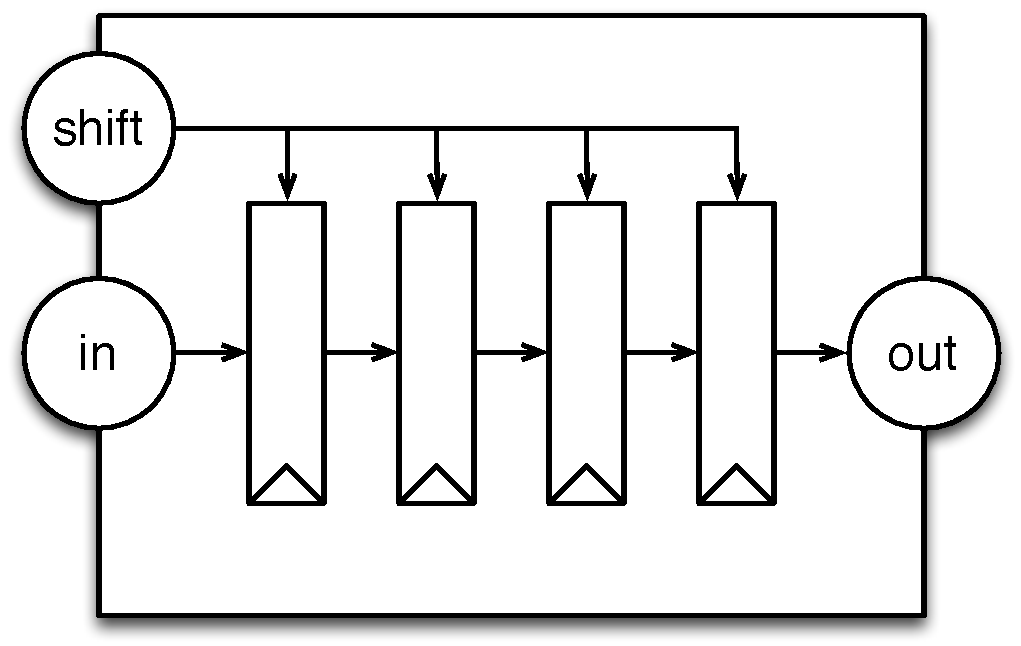
\includegraphics[width=0.9\textwidth]{figs/enable-shift-register.pdf}
\end{center}

\end{columns}

\end{frame}

\begin{frame}[fragile]{Conditional Register Update with Reset}

\begin{scala}
class EnableShiftRegister extends Module {
  val io = new Bundle {
    val in    = UInt(INPUT, 1)
    val shift = Bool(INPUT)
    val out   = UInt(OUTPUT, 1)
  }
  // Register reset to zero
  val r0 = Reg(init = UInt(0, 1))
  val r1 = Reg(init = UInt(0, 1))
  val r2 = Reg(init = UInt(0, 1))
  val r3 = Reg(init = UInt(0, 1))
  when (io.shift) {
    r0 := io.in
    r1 := r0
    r2 := r1
    r3 := r2
  }
  io.out := r3
}
\end{scala}

\end{frame}

\begin{frame}[fragile]{UInt Literals}
inferred width
\begin{scala}
UInt(1)       // decimal 1-bit literal from Scala Int. 
UInt("ha")    // hexadecimal 4-bit literal from string.
UInt("o12")   // octal 4-bit literal from string. 
UInt("b1010") // binary 4-bit literal from string.
\end{scala}
specified widths
\begin{scala}
UInt("h_dead_beef") // 32-bit literal of type UInt.
UInt(1)             // decimal 1-bit literal from Scala Int.
UInt("ha", 8)       // hexadecimal 8-bit literal of type UInt.
UInt("o12", 6)      // octal 6-bit literal of type UInt.
UInt("b1010", 12)   // binary 12-bit literal of type UInt.
UInt(5, 8)          // unsigned decimal 8-bit literal of type UInt.
\end{scala}
\end{frame}


\setbeamercolor{frametitle}{bg=\frametitleproblemcolor}
\begin{frame}[fragile]{Sequential Circuit Problem -- \tt Accumulator.scala}
\begin{itemize}
\item write sequential circuit that sums \code{in} values
\item in {\tt chisel-tutorial/problems/Accumulator.scala}
\item run {\tt make Accumulator.out} until passing
\end{itemize}
\begin{scala}
class Accumulator extends Module {
  val io = new Bundle {
    val in  = UInt(INPUT, 1)
    val out = UInt(OUTPUT, 8)
  }

  // flush this out ...

  io.out := UInt(0)
}
\end{scala}
\end{frame}
\setbeamercolor{frametitle}{bg=\frametitledefaultcolor}

\begin{frame}[fragile]{UInt Operations and Conditional Assignment}

\begin{columns}
\column{0.5\textwidth}

{\lstset{basicstyle={\tiny\ttfamily}}
\begin{scala}
class BasicALU extends Module {
  val io = new Bundle {
    val a      = UInt(INPUT, 4)
    val b      = UInt(INPUT, 4)
    val opcode = UInt(INPUT, 4)
    val output = UInt(OUTPUT, 4)
  }
  io.output := UInt(0) 
  when (io.opcode === UInt(0)) {
    io.output := io.a                   // pass A
  } .elsewhen (io.opcode === UInt(1)) {
    io.output := io.b                   // pass B
  } .elsewhen (io.opcode === UInt(2)) {
    io.output := io.a + UInt(1)         // inc A by 1
  } .elsewhen (io.opcode === UInt(3)) {
    io.output := io.a - UInt(1)         // dec B by 1
  } .elsewhen (io.opcode === UInt(4)) {
    io.output := io.a + UInt(4)         // inc A by 4
  } .elsewhen (io.opcode === UInt(5)) {
    io.output := io.a - UInt(4)         // dec A by 4
  } .elsewhen (io.opcode === UInt(6)) {
    io.output := io.a + io.b            // add A and B
  } .elsewhen (io.opcode === UInt(7)) {
    io.output := io.a - io.b            // sub B from A
  } .elsewhen (io.opcode === UInt(8)) {
    io.output := (io.a < io.b)          // set on A < B
  } .otherwise { 
    io.output := (io.a === io.b)        // set on A == B
  }
}
\end{scala}
}

\column{0.4\textwidth}
\begin{itemize}
\item wire \code{io.output} defaulted to 0 and then
\item conditionally reassigned to based on opcode
\item unlike registers, wires are required to be defaulted
\item wires also allow forward declarations
\end{itemize}
\end{columns}
\end{frame}

\begin{frame}[fragile]{UInt Operations}

\begin{center}
\begin{tabular}{| c | c | c | }
\hline
Symbol & Operation & Output Type \\ \hline
\verb!+! & Add & UInt  \\ \hline
\verb+-+ & Subtract & UInt  \\ \hline
\verb+*+ & Multiply & UInt \\ \hline
\verb+/+ & UInt Divide & UInt \\ \hline
\verb+%+ & Modulo & UInt \\ \hline
\verb+~+ & Bitwise Negation & UInt \\ \hline
\verb+^+ & Bitwise XOR & UInt\\ \hline
\verb+&+ & Bitwise AND & UInt \\ \hline
\verb+|+ & Bitwise OR & Bool \\ \hline
{\color{red}\verb+===+} & Equal & Bool \\ \hline
\verb+!=+ & Not Equal & Bool \\ \hline
\verb+>+ & Greater & Bool \\ \hline
\verb+<+ & Less & Bool \\ \hline
\verb+>=+ & Greater or Equal & Bool \\ \hline
\verb+<=+ & Less or Equal & Bool \\ \hline
\end{tabular}
\end{center}

\end{frame}

\begin{frame}[fragile]{Bit Extraction}
\begin{scala}
// extracts the x through y bits of value
val x_to_y = value(x, y) 
\end{scala}

\begin{scala}
// extract the x-th bit from value
val x_of_value = value(x)
\end{scala}
\end{frame}

\begin{frame}[fragile]{ByteSelector}

\begin{scala}
class ByteSelector extends Module {
  val io = new Bundle {
    val in     = UInt(INPUT, 32)
    val offset = UInt(INPUT, 2)
    val out    = UInt(OUTPUT, 8)
  }
  io.out := UInt(0, width = 8)
  when (io.offset === UInt(0)) {
    io.out := io.in(7,0)   // pull out lowest byte
  } .elsewhen (io.offset === UInt(1)) {
    io.out := io.in(15,8)  // pull out second byte
  } .elsewhen (io.offset === UInt(2)) {
    io.out := io.in(23,16) // pull out third byte
  } .otherwise {
    io.out := io.in(31,24) // pull out highest byte
  }    
}
\end{scala}

\end{frame}

% \setbeamercolor{frametitle}{bg=\frametitleproblemcolor}
% \begin{frame}[fragile]{Instruction Decoder}
% 
% {\lstset{basicstyle={\scriptsize\ttfamily}}
% \begin{scala}
% class LoadShiftRegister extends Module {
%   val io = new Bundle {
%     val inst  = UInt(INPUT, 32)
%     val rs0   = UInt(OUTPUT, 8)
%     val rs1   = UInt(OUTPUT, 8)
%     val rs2   = UInt(OUTPUT, 8)
%     val isAdd = Bool(OUTPUT)
%     val isSub = Bool(OUTPUT)
%     val isMul = Bool(OUTPUT)
%     val isDiv = Bool(OUTPUT)
%   }
%   io.isAdd := ...
%   io.isSub := ...
%   io.isMul := ...
%   io.isDiv := ...
%   io.rs0   := ...
%   io.rs1   := ...
%   io.rs2   := ...
% }
% \end{scala}
% }
% 
% \end{frame}
% \setbeamercolor{frametitle}{bg=\frametitledefaultcolor}

\begin{frame}[fragile]{Bit Concatenation and Filling}
You concatenating bits using \verb+Cat+:
\begin{scala}
val A   = UInt(width = 32)
val B   = UInt(width = 32)
val bus = Cat(A, B) // concatenate A and B
\end{scala}

and replicate bits using \verb+Fill+:
\begin{scala}
// Replicate a bit string multiple times.
val usDebt = Fill(3, UInt("hA")) 
\end{scala}

\end{frame}

\setbeamercolor{frametitle}{bg=\frametitleproblemcolor}
\begin{frame}[fragile]{LFSR16 -- \tt problems/lfsr16.scala}

\begin{scala}
class LFSR16 extends Module {
  val io = new Bundle {
    val inc = Bool(INPUT)
    val out = UInt(OUTPUT, 16)
  }
  // ...
  io.out := UInt(0)
}
\end{scala}
\begin{itemize}
\item \verb+reg+, \verb+cat+, \verb+extract+, \verb+^+
\item init reg to 1
\item updates when \verb+inc+ asserted
\end{itemize}

\begin{center}
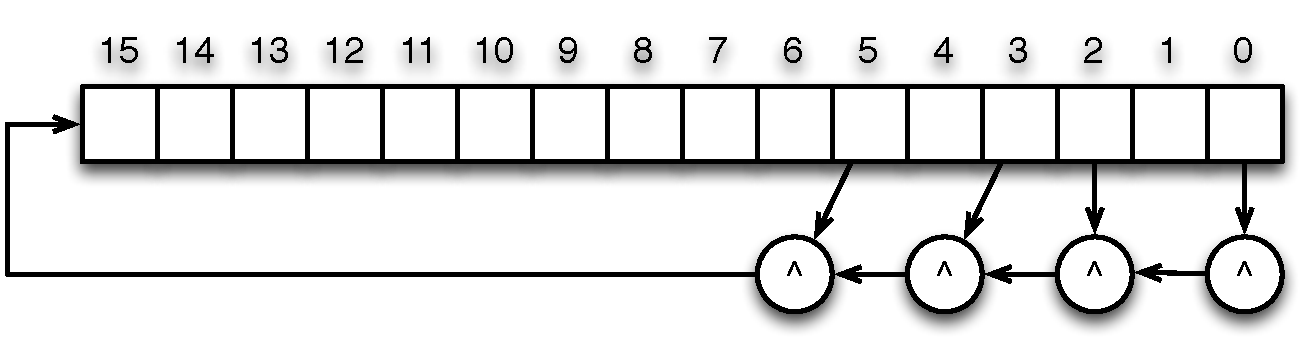
\includegraphics[width=0.9\textwidth]{figs/LFSR16.pdf}
\end{center}

\end{frame}
\setbeamercolor{frametitle}{bg=\frametitledefaultcolor}

\begin{frame}[fragile]{UInt Bit Inference}
\begin{columns}
\column{0.4\textwidth}
\begin{scala}
class HiLoMultiplier() 
    extends Module {
  val io = new Bundle {
    val A  = UInt(INPUT, 16)
    val B  = UInt(INPUT, 16)
    val Hi = UInt(OUTPUT, 16)
    val Lo = UInt(OUTPUT, 16)
  }
  val mult = io.A * io.B
  io.Lo := mult(15, 0)
  io.Hi := mult(31, 16)  
}
\end{scala}

\column{0.5\textwidth}

{\lstset{basicstyle={\scriptsize\ttfamily}}
\begin{scala}
module HiLoMultiplier(
    input [15:0] io_A,
    input [15:0] io_B,
    output[15:0] io_Hi,
    output[15:0] io_Lo);

  wire[15:0] T0;
  wire[31:0] mult; // inferred as 32 bits
  wire[15:0] T1;

  assign io_Lo = T0;
  assign T0 = mult[4'hf:1'h0];
  assign mult = io_A * io_B;
  assign io_Hi = T1;
  assign T1 = mult[5'h1f:5'h10];
endmodule
\end{scala}
}

\end{columns}

\end{frame}

\begin{frame}[fragile]{Bit Inference Rules}

\begin{center}
\begin{tabular}{| l | l | l | }
\hline
Operation & Result Bit Width \\ \hline
\verb!Z = X + Y! & max(Width(X), Width(Y))  \\ \hline
\verb+Z = X - Y+ & max(Width(X), Width(Y)) \\ \hline
\verb+Z = X & Y+ & min(Width(X), Width(Y)) \\ \hline
\verb+Z = X | Y+ & max(Width(X), Width(Y)) \\ \hline
\verb+Z = X ^ Y+ & max(Width(X), Width(Y)) \\ \hline
\verb+Z = ~X+ & Width(X) \\ \hline
\verb+Z = Mux(C, X, Y)+ & max(Width(X), Width (Y)) \\ \hline
\verb+Z = X * Y+ & Width(X) + Width(Y) \\ \hline
\verb+Z = X << n+ & Width(X) + n \\ \hline
\verb+Z = X >> n+ & Width(X) - n \\ \hline
\verb+Z = Cat(X, Y)+ & Width(X) + Width(Y) \\ \hline
\verb+Z = Fill(n, x)+ & Width(X) + n \\ \hline
\end{tabular}
\end{center}

\end{frame}

\begin{frame}[fragile]{Bool Type}
The Chisel Bool is used to represent the result of logical expressions:
\begin{scala}
val change = io.a === io.b // change gets Bool type
when (change) { // execute if change is true
 ...
} 
\end{scala}

You can instantiate a Bool value like this:
\begin{scala}
val true_value  = Bool(true)
val false_value = Bool(false)
\end{scala}

You can cast an UInt to a Bool as follows:
\begin{scala}
val bit = UInt(width = 1) ...
when (bit.toBool) { ... }
\end{scala}

You can use a Bool as an UInt:
\begin{scala}
val bit = UInt(width = 1) ...
bit := a > b
\end{scala}

\end{frame}

\begin{frame}[fragile]{Bits Subtype Hierarchy}
\begin{itemize}
\item \verb+SInt+ is a signed integer type
\end{itemize}
\begin{center}
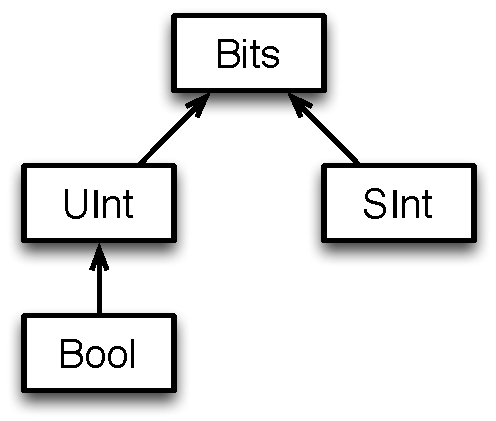
\includegraphics[height=0.7\textheight]{figs/bits-hierarchy.pdf}
\end{center}
\end{frame}

\begin{frame}[fragile]{Bundles}

\begin{columns}
\column{0.55\textwidth}
\begin{scala}
class MyFloat extends Bundle {
  val sign        = Bool()
  val exponent    = UInt(width = 8)
  val significand = UInt(width = 23)
}

val x  = new MyFloat()
val xs = x.sign
\end{scala}

\column{0.35\textwidth}

\begin{center}
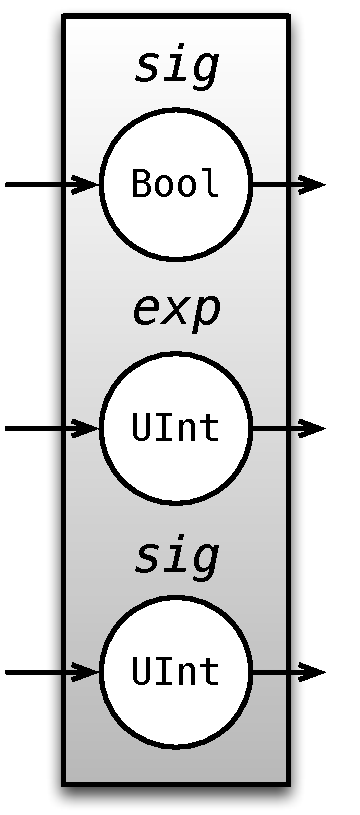
\includegraphics[height=0.9\textheight]{../cs250/figs/myfloat.pdf} 
\end{center}

\end{columns}
\end{frame}

\begin{frame}[fragile]{Ports}

\begin{columns}
\column{0.55\textwidth}

\textbf{Data object with directions assigned to its members}

\begin{scala}
class Decoupled extends Bundle {
  val data  = UInt(INPUT, 32)
  val valid = Bool(OUTPUT)
  val ready = Bool(INPUT)
}
\end{scala}

\textbf{Direction assigned at instantiation time}

\begin{scala}
class ScaleIO extends Bundle {
  val in    = new MyFloat().asInput
  val scale = new MyFloat().asInput
  val out   = new MyFloat().asOutput
}
\end{scala}

\column{0.35\textwidth}

\begin{center}
\includegraphics[height=0.9\textheight]{../cs250/figs/fifoio.pdf} 
\end{center}

\end{columns}

\end{frame}

\begin{frame}[fragile]{Instantiating Modules}

\begin{columns}

\column{0.4\textwidth}

{\lstset{basicstyle={\tiny\ttfamily}}
\begin{scala}
// A 4-bit adder with carry in and carry out
class Adder4 extends Module {
  val io = new Bundle {
    val A    = UInt(INPUT, 4)
    val B    = UInt(INPUT, 4)
    val Cin  = UInt(INPUT, 1)
    val Sum  = UInt(OUTPUT, 4)
    val Cout = UInt(OUTPUT, 1)
  }
  // Adder for bit 0
  val Adder0 = Module(new FullAdder())
  Adder0.io.a   := io.A(0)
  Adder0.io.b   := io.B(0)
  Adder0.io.cin := io.Cin
  val s0 = Adder0.io.sum
  // Adder for bit 1
  val Adder1 = Module(new FullAdder())
  Adder1.io.a   := io.A(1)
  Adder1.io.b   := io.B(1)
  Adder1.io.cin := Adder0.io.cout
  val s1 = Cat(Adder1.io.sum, s0)
  ...
  // Adder for bit 3
  val Adder3 = Module(new FullAdder())
  Adder3.io.a   := io.A(3)
  Adder3.io.b   := io.B(3)
  Adder3.io.cin := Adder2.io.cout
  io.Sum  := Cat(Adder3.io.sum, s2)
  io.Cout := Adder3.io.cout
}
\end{scala}
}

\column{0.5\textwidth}

\begin{center}
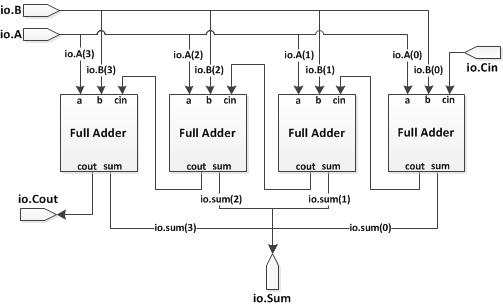
\includegraphics[width=0.9\textwidth]{../getting-started/figs/4_Bit_Adder.jpg}
\end{center}

\begin{itemize}
\item inherits from \verb+Module+ class,
\item contains an interface stored in a port field named \verb+io+, and
\item wires together subcircuits in its constructor.
\end{itemize}

\end{columns}

\end{frame}

\begin{frame}[fragile]{Vecs}
constructing vecs
\begin{scala}
val myVec1 = Vec.fill( <number of elements> ) { <data type> }
val myVec2 = Vec(<elt0>, <elt1>, ...)
\end{scala}

creating a vec of wires
\begin{scala}
val ufix5_vec10 = Vec.fill(10) { UInt(width = 5) }
\end{scala}


creating a vec of regs
\begin{scala}
val reg_vec32 = Vec.fill(32){ Reg() }
\end{scala}

writing
\begin{scala}
reg_vec32(1) := UInt(0)
\end{scala}

reading
\begin{scala}
val reg5 = reg_vec(5)
\end{scala}

\end{frame}

\setbeamercolor{frametitle}{bg=\frametitleproblemcolor}
\begin{frame}[fragile]{Vec Shift Reg -- problems/VecShiftRegister.scala}

\begin{itemize}
\item add loadability to shift register
\item change interface to use vec's
\end{itemize}

{\lstset{basicstyle={\scriptsize\ttfamily}}
\begin{scala}
class VecShiftRegister extends Module {
  val io = new Bundle {
    val ins   = Vec.fill(4){ UInt(INPUT, 1) }
    val load  = Bool(INPUT)
    val shift = Bool(INPUT)
    val out   = UInt(OUTPUT, 4)
  }
  val delays = Vec.fill(4){ Reg(UInt(width = 4)) }
  when ( ... ) {
  // fill in here ...
  } .elsewhen (io.shift) {
    ...
  }
  io.out := delays(3)
}
\end{scala}
}

\end{frame}
\setbeamercolor{frametitle}{bg=\frametitledefaultcolor}

% \begin{frame}[fragile]{Scala Console}
% \begin{FramedVerb}
% \end{FramedVerb}
% \end{frame}

\begin{frame}[fragile]{Defining a Tester}

\begin{columns}
\column{0.45\textwidth}
{\lstset{basicstyle={\tiny\ttfamily}}
\begin{scala}
package Tutorial
import Chisel._

class ByteSelector extends Module {
  val io = new Bundle {
    val in     = UInt(INPUT, 32)
    val offset = UInt(INPUT, 2)
    val out    = UInt(OUTPUT, 8)
  }
  io.out := UInt(0, width=8)
  ...
}

class BSTests(c: ByteSelector) extends Tester(c) {
  val test_in = 12345678
  for (t <- 0 until 4) {
    poke(c.io.in, test_in)
    poke(c.io.offset, t)
    step(1)
    val ref_out = (test_in >> (t * 8)) & 0xFF
    expect(c.io.out, ref_out)
  }
}
\end{scala}
}
\begin{center}
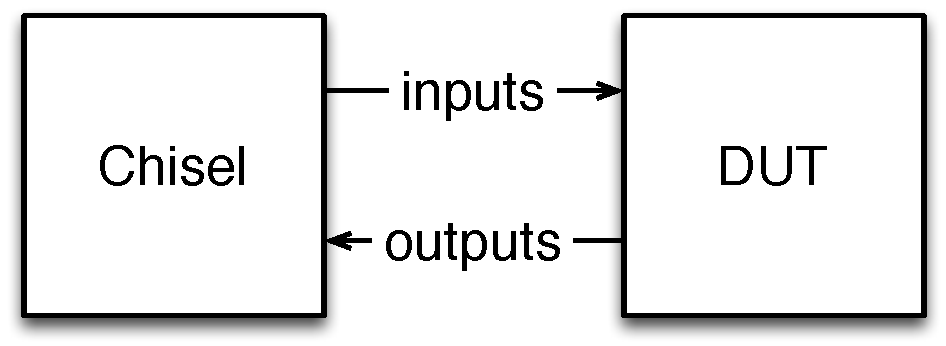
\includegraphics[width=0.8\textwidth]{../tutorial/figs/DUT.pdf}
\end{center}

\column{0.45\textwidth}
{\lstset{basicstyle={\tiny\ttfamily}}
\begin{scala}
class Tester[T <: Module]
    (val c: T, val isTrace: Boolean = true) {
  var t: Int
  var ok: Boolean
  val rnd: Random
  def reset(n: Int = 1)
  def step(n: Int): Int
  def peek(data: Aggregate): Array[BigInt]
  def peekAt(data: Mem[T], index: Int)
  def peek(data: Bits): BigInt
  def int(x: Boolean): BigInt
  def int(x: Int): BigInt
  def int(x: Bits): BigInt
  def poke(data: Aggregate, x: Array[BigInt])
  def pokeAt(data: Mem[T], index: Int, x: BigInt)
  def poke(data: Bits, x: BigInt)
  def expect (good: Boolean, msg: String): Boolean
  def expect (data: Bits, target: BigInt): Boolean
}
\end{scala}
}
\begin{tiny}
\noindent
which binds a tester to a module
and allows users to write tests using the given debug protocol.  In particular, users utilize:
\begin{itemize}
\item \code{poke} to set input port and state values,
\item \code{step} to execute the circuit one time unit,
\item \code{peek} to read port and state values, and
\item \code{expect} to compare peeked circuit values to expected arguments.
\end{itemize}
\end{tiny}

\end{columns}
\end{frame}

\begin{frame}[fragile]{Simulation Debug Output}

{\lstset{basicstyle={\tiny\ttfamily}}
\begin{scala}
> cd chisel-tutorial/examples
> make ByteSelector.out
STARTING ../emulator/problems/ByteSelector
---
INPUTS
  INPUT(ByteSelector__io_in.ByteSelector) = 12345678
  INPUT(ByteSelector__io_offset.ByteSelector) = 0
OUTPUTS
  READ OUTPUT(ByteSelector__io_out.ByteSelector) = 78
  EXPECTED: OUTPUT(ByteSelector__io_out.ByteSelector) = 78
  SUCCESS
---
INPUTS
  INPUT(ByteSelector__io_in.ByteSelector) = 12345678
  INPUT(ByteSelector__io_offset.ByteSelector) = 1
OUTPUTS
  READ OUTPUT(ByteSelector__io_out.ByteSelector) = 97
  EXPECTED: OUTPUT(ByteSelector__io_out.ByteSelector) = 97
  SUCCESS
---
...
---
INPUTS
  INPUT(ByteSelector__io_in.ByteSelector) = 12345678
  INPUT(ByteSelector__io_offset.ByteSelector) = 3
OUTPUTS
  READ OUTPUT(ByteSelector__io_out.ByteSelector) = 0
  EXPECTED: OUTPUT(ByteSelector__io_out.ByteSelector) = 0
  SUCCESS
PASSED   // Final pass assertion
[success] Total time: 26 s, ...
\end{scala}
}

\end{frame}

\begin{frame}{Testbench Ingredients}

In particular, users utilize:
\begin{itemize}
\item \code{poke} to set input port and state values,
\item \code{step} to execute the circuit one time unit,
\item \code{peek} to read port and state values, and
\item \code{expect} to compare peeked circuit values to expected arguments.
\end{itemize}

\end{frame}

\setbeamercolor{frametitle}{bg=\frametitleproblemcolor}
\begin{frame}[fragile]{Testbench for MaxN -- \tt MaxN.scala}
\begin{columns}
\column{0.49\textwidth}

\begin{itemize}
\item write a testbench for MaxN
\end{itemize}

{\lstset{basicstyle={\scriptsize\ttfamily}}
\begin{scala}
class MaxN(val n: Int, val w: Int) 
    extends Module {

  def Max2(x: UInt, y: UInt) = 
    Mux(x > y, x, y)

  val io = new Bundle {
    val ins = Vec.fill(n){ UInt(INPUT, w) }
    val out = UInt(OUTPUT, w)
  }
  io.out := io.ins.reduceLeft(Max2)
}
\end{scala}
}
\begin{scala}
// returns random int in 0..lim-1
val x = rnd.nextInt(lim) 
\end{scala}

\column{0.42\textwidth}

{\lstset{basicstyle={\scriptsize\ttfamily}}
\begin{scala}
class MaxNTests(c: MaxN) extends Tester(c) {
  for (i <- 0 until 10) {
    for (j <- 0 until c.n) {
      // FILL THIS IN HERE
      poke(c.io.ins(0), 0)
    }
    // FILL THIS IN HERE
    step(1)
    expect(c.io.out, 1)
  }
}
\end{scala}
}
\end{columns}
\end{frame}
\setbeamercolor{frametitle}{bg=\frametitledefaultcolor}

\begin{frame}[fragile]{Dynamically Accessed Vec}
\begin{scala}
class MemorySearch extends Module {
  val io = new Bundle {
    val target  = UInt(INPUT,  4)
    val en      = Bool(INPUT)
    val address = UInt(OUTPUT, 3)
    val done    = Bool(OUTPUT)
  }
  val index  = Reg(init = UInt(0, width = 3))
  val list   = Vec(UInt(0), UInt(4), UInt(15), UInt(14), 
                   UInt(2), UInt(5), UInt(13)){ UInt(width = 4) }
  val memVal = list(index)
  val done   = !io.en && ((memVal === io.target) || (index === UInt(7)))
  when (io.en) {
    index := UInt(0)
  } .elsewhen (done === Bool(false)) {
    index := index + UInt(1)
  }
  io.done    := done
  io.address := index
}
\end{scala}
\end{frame}

\begin{frame}[fragile]{RAM}
RAM is supported using the \code{Mem} construct

\begin{scala}
val m = Mem(Bits(width = 32), 32)
\end{scala}

\noindent
where
\begin{itemize}
\item writes to Mems are positive-edge-triggered
\item reads are either combinational or positive-edge-triggered
\item ports are created by applying a \code{UInt} index
\end{itemize}
\end{frame}

\begin{frame}[fragile]{32-entry Register File}

\begin{scala}
val regs = Mem(Bits(width = 32), 32)
when (wrEn) {
  regs(wrAddr) := wrData
}
val iDat = regs(iAddr)
val mDat = regs(mAddr)
\end{scala}

\begin{center}
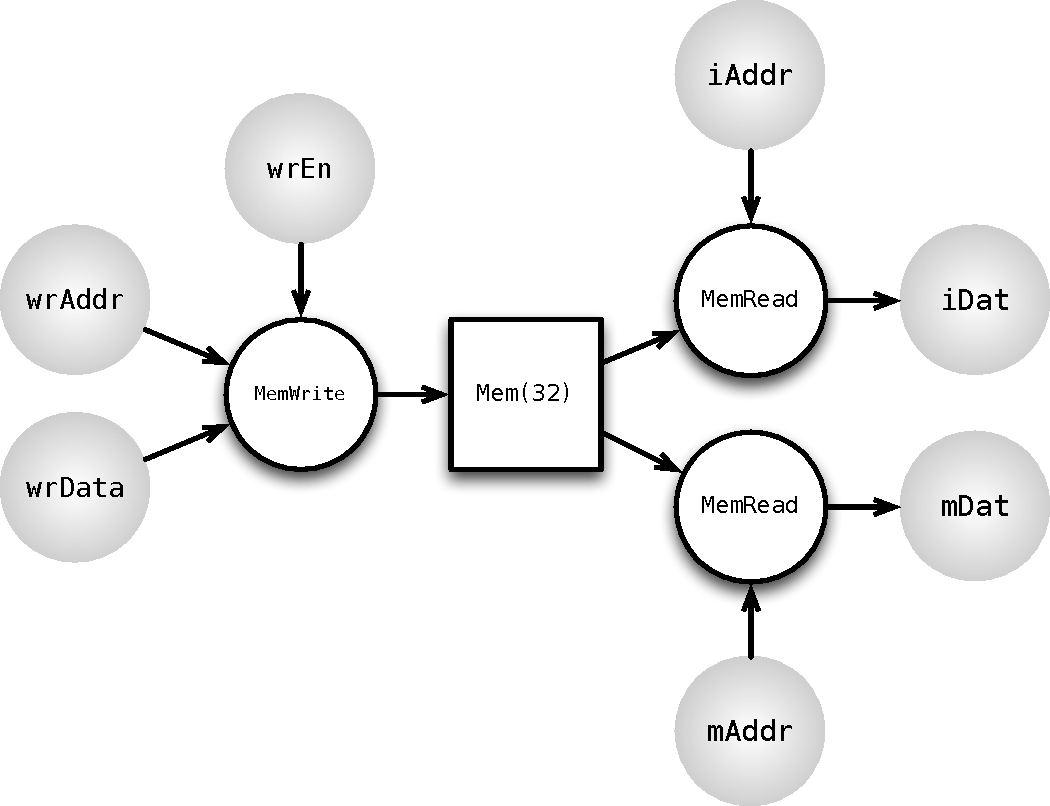
\includegraphics[height=0.55\textheight]{../cs250/figs/mem.pdf} 
\end{center}

\end{frame}

\setbeamercolor{frametitle}{bg=\frametitleproblemcolor}
\begin{frame}[fragile]{Load/Search Mem -- \tt DynamicMemorySearch.scala}
\begin{scala}
class DynamicMemorySearch extends Module {
  val io = new Bundle {
    val isWr   = Bool(INPUT)
    val wrAddr = UInt(INPUT,  3)
    val data   = UInt(INPUT,  4)
    val en     = Bool(INPUT)
    val target = UInt(OUTPUT, 3)
    val done   = Bool(OUTPUT)
  }
  val index  = Reg(init = UInt(0, width = 3))
  val memVal = ...
  val done = !io.en && ((memVal === io.data) || (index === UInt(7)))
  // ...
  when (io.en) {
    index := UInt(0)
  } .elsewhen (done === Bool(false)) {
    index := index + UInt(1)
  }
  io.done   := done
  io.target := index
}
\end{scala}
\end{frame}
\setbeamercolor{frametitle}{bg=\frametitledefaultcolor}

\begin{frame}[fragile]{Sequential Read Ports}
Sequential read ports are inferred when:
\begin{itemize}
\item optional parameter \code{seqRead} is set and
\item read address is a reg
\end{itemize}

\begin{scala}
val ram1r1w = Mem(UInt(width = 32), 1024, seqRead = true)
val reg_raddr = Reg(UInt())
when (wen) { ram1r1w(waddr) := wdata }
when (ren) { reg_raddr := raddr }
val rdata = ram1r1w(reg_raddr)
\end{scala}

\begin{center}
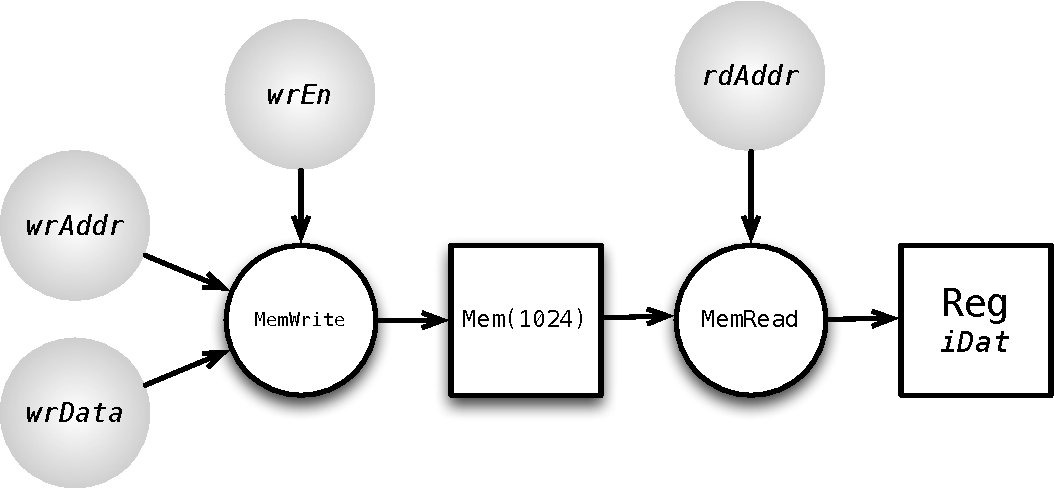
\includegraphics[height=0.4\textheight]{../cs250/figs/mem-seq-read.pdf} 
\end{center}

\end{frame}

\begin{frame}[fragile]{Stack}

{\lstset{basicstyle={\tiny\ttfamily}}
\begin{scala}
class Stack(depth: Int) extends Module {
  val io = new Bundle {
    val dataIn  = UInt(INPUT,  32)
    val dataOut = UInt(OUTPUT, 32)
    val push    = Bool(INPUT)
    val pop     = Bool(INPUT)
    val en      = Bool(INPUT)
  }
  // declare the memory for the stack
  val stack_mem = Mem(UInt(width = 32), depth, seqRead = false)
  val sp = Reg(init = UInt(0, width = log2Up(depth)))
  val dataOut = Reg(init = UInt(0, width = 32))
  // Push condition - make sure stack isn't full
  when(io.en && io.push && (sp != UInt(depth-1))) {
    stack_mem(sp + UInt(1)) := io.dataIn
    sp := sp + UInt(1)
  } 
  // Pop condition - make sure the stack isn't empty
  .elsewhen(io.en && io.pop && (sp > UInt(0))) {
    sp := sp - UInt(1)
  }
  when(io.en) {
    dataOut := stack_mem(sp)
  }
  io.dataOut := dataOut
}
\end{scala}
}

\end{frame}

\begin{frame}[fragile]{Scripting Hardware Generation}

\begin{columns}
\column{0.5\textwidth}

{\lstset{basicstyle={\tiny\ttfamily}}
\begin{scala}
// A n-bit adder with carry in and carry out
class Adder(n: Int) extends Module {
  val io = new Bundle {
    val A    = UInt(INPUT, n)
    val B    = UInt(INPUT, n)
    val Cin  = UInt(INPUT, 1)
    val Sum  = UInt(OUTPUT, n)
    val Cout = UInt(OUTPUT, 1)
  }
  // create a vector of FullAdders
  val FAs   = Vec.fill(n){ Module(new FullAdder()).io }
  val carry = Vec.fill(n+1){ UInt(width = 1) }
  val sum   = Vec.fill(n){ Bool() }

  // first carry is the top level carry in
  carry(0) := io.Cin

  // wire up the ports of the full adders
  for(i <- 0 until n) {
    FAs(i).a   := io.A(i)
    FAs(i).b   := io.B(i)
    FAs(i).cin := carry(i)
    carry(i+1) := FAs(i).cout
    sum(i)     := FAs(i).sum.toBool()
  }
  io.Sum  := sum.toBits().toUInt()
  io.Cout := carry(n)
}
\end{scala}
}

\column{0.4\textwidth}

\begin{center}
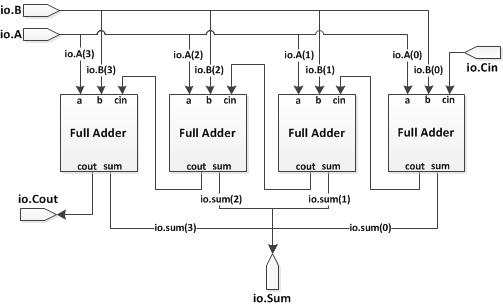
\includegraphics[width=0.9\textwidth]{../getting-started/figs/4_Bit_Adder.jpg}
\end{center}
\end{columns}

\end{frame}

% \begin{frame}[fragile]{Chisel Today}
% \begin{itemize}
% \item whirlwind tour of chisel
% \item recents results and products
% \item update on upcoming release
% \item future research work
% \end{itemize}
% \end{frame}

\begin{frame}[fragile]
\frametitle{What is Chisel?}
\vfill
\begin{itemize}
\item {\bf Abstractly}: Chisel is a framework for {\it programmatically} generating circuitry.
\item {\bf Less Abstractly}: Chisel is a software library for creating and connecting circuit components to form a circuit graph.
\item {\bf Concretely}: Chisel is a DSL embedded in Scala for creating and connecting circuit components, with tools for simulation and translation to Verilog.
\end{itemize}
\vspace{3.5cm}
{\it\small * based on slides by my PhD student Patrick Li}
\end{frame}

\begin{frame}[fragile]
\frametitle{Chisel is a {\it Library}}
\begin{itemize}
\item Classes are provided for circuit components:
\begin{itemize}
\item \verb+Register()+
\item \verb+Adder()+
\item \verb+Multiplexor()+
\item \verb+Wire(name)+
\item \verb+Constant(name)+
\end{itemize}

\noindent
and \verb+new+ used to construct components and \verb+connect+ used to wire them together:
\begin{itemize}
\item \verb+new Register()+
\item ...
\item \verb+connect(input, output)+
\end{itemize}
\end{itemize}
\end{frame}

\begin{frame}[fragile]
\frametitle{What if Chisel was a Scala Library?}
\begin{columns}
\column{0.50\textwidth}
{\lstset{basicstyle={\tiny\ttfamily}}
\begin{scala}
def main(args: Array[String]) = {
  // Create Components
  val reset       = new Wire("reset");
  val counter     = new Register("counter");
  val adder       = new Adder();
  val multiplexor = new Multiplexor();
  val one         = new UInt(1);
  val zero        = new UInt(0);

  // Connect Components
  connect(multiplexor.choice, reset);
  connect(multiplexor.in_a, zero.out);
  connect(multiplexor.in_b, adder.out);
  connect(counter.in, multiplexor.out);
  connect(adder.in_a, counter.out);
  connect(adder.in_b, one.out);

  // Produce Verilog
  generate_verilog(counter);
}
\end{scala}
}
\column{0.40\textwidth}
\begin{center}
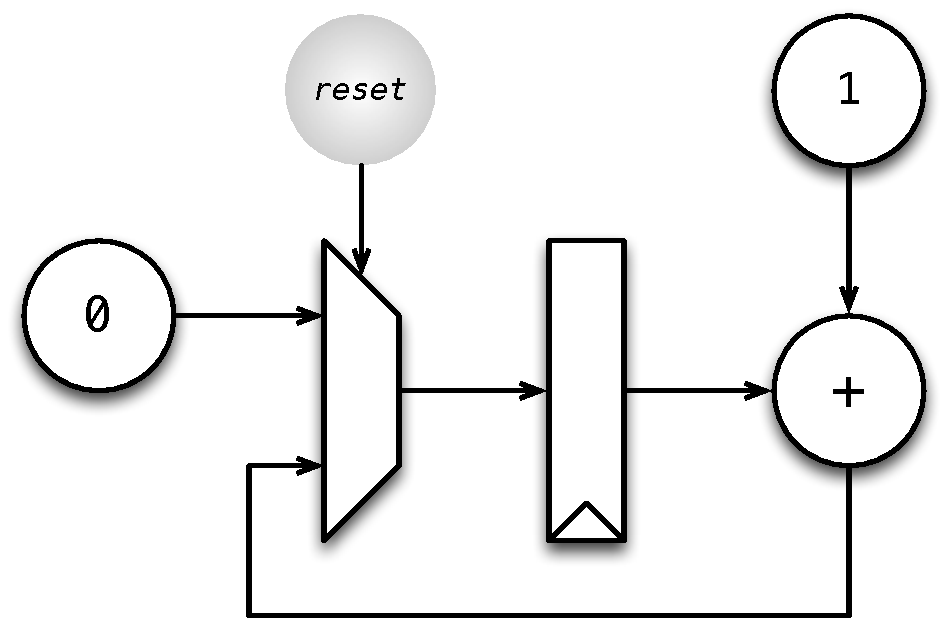
\includegraphics[width=0.9\textwidth]{figs/simple-counter.pdf}
\end{center}
\end{columns}
\end{frame}

\begin{frame}[fragile]
\frametitle{What if Chisel was a Scala Library?}
\begin{columns}
\column{0.50\textwidth}
{\lstset{basicstyle={\tiny\ttfamily}}
\begin{scala}
def main(args: Array[String]) = {
  // Create Components
  val reset       = new Wire("reset");
  val counter     = new Register("counter");
  val adder       = new Adder();
  val multiplexor = new Multiplexor();
  val one         = new UInt(1);
  val zero        = new UInt(0);

  // Connect Components
  connect(multiplexor.choice, reset);
  connect(multiplexor.in_a, zero.out);
  connect(multiplexor.in_b, adder.out);
  connect(counter.in, multiplexor.out);
  connect(adder.in_a, counter.out);
  connect(adder.in_b, one.out);

  // Produce Verilog
  generate_verilog(counter);
}
\end{scala}
}
\column{0.40\textwidth}
\begin{center}
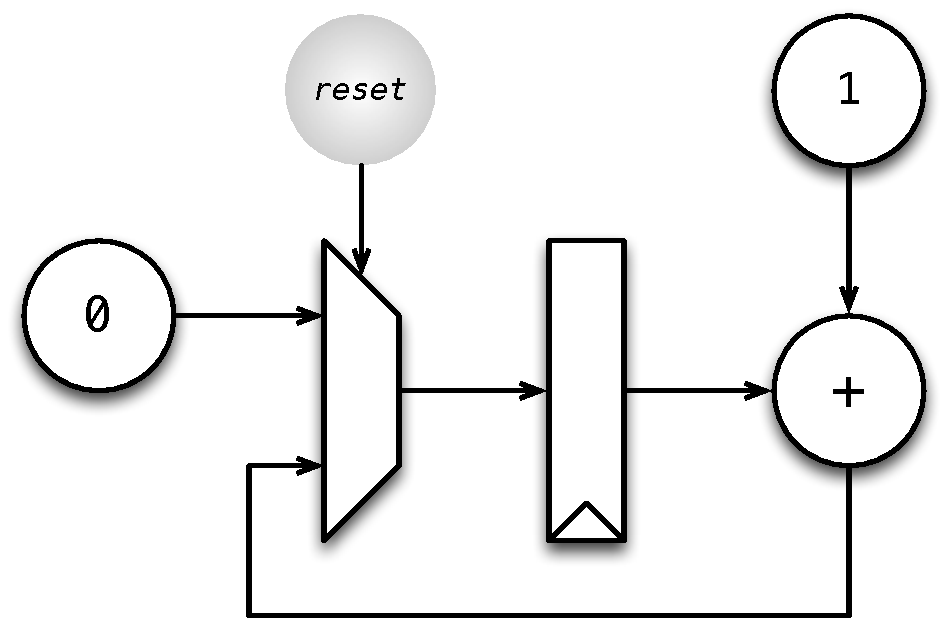
\includegraphics[width=0.9\textwidth]{figs/simple-counter.pdf}
\end{center}
\end{columns}
\begin{itemize}
\item using Scala to programmatically generate hardware
\item can use full power of Scala (loops, arrays, conditionals, ...)
\end{itemize}
\end{frame}

\begin{frame}[fragile]
\frametitle{What if Chisel was a Scala Library?}
\begin{columns}
\column{0.50\textwidth}
{\lstset{basicstyle={\tiny\ttfamily}}
\begin{scala}
def main(args: Array[String]) = {
  // Create Components
  val reset       = new Wire("reset");
  val counter     = new Register("counter");
  val adder       = new Adder();
  val multiplexor = new Multiplexor();
  val one         = new UInt(1);
  val zero        = new UInt(0);

  // Connect Components
  connect(multiplexor.choice, reset);
  connect(multiplexor.in_a, zero.out);
  connect(multiplexor.in_b, adder.out);
  connect(counter.in, multiplexor.out);
  connect(adder.in_a, counter.out);
  connect(adder.in_b, one.out);

  // Produce Verilog
  generate_verilog(counter);
}
\end{scala}
}
\column{0.40\textwidth}
\begin{center}
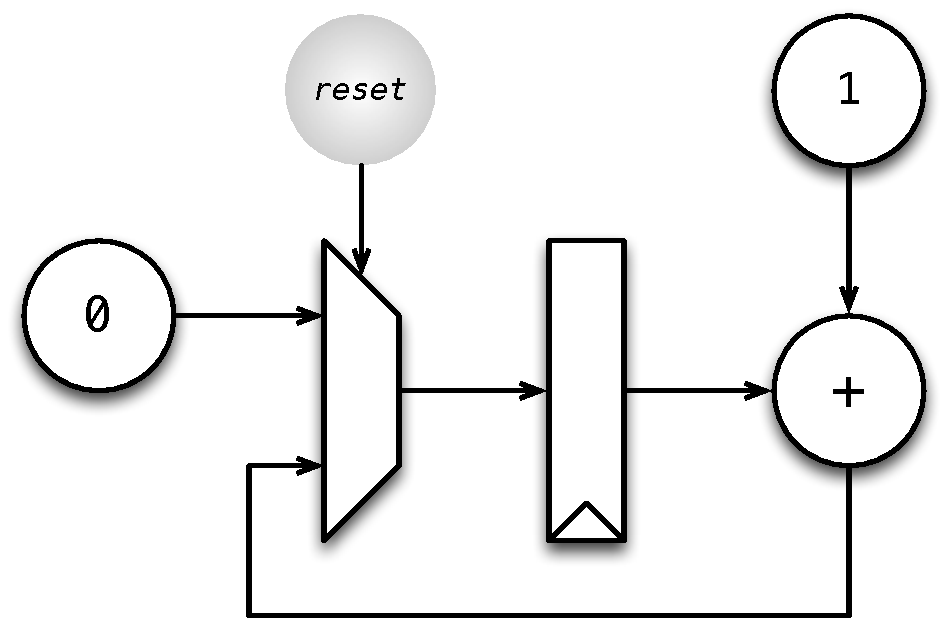
\includegraphics[width=0.9\textwidth]{figs/simple-counter.pdf}
\end{center}
\end{columns}
\begin{itemize}
\item but Scala is pretty Verbose, how can we do better?
\end{itemize}
\end{frame}

\begin{frame}[fragile]
\frametitle{Functional Composition of Adder}
\begin{columns}
\column{0.4\textwidth}
{\lstset{basicstyle={\tiny\ttfamily}}
\begin{scala}
def main(args: Array[String]) = {
  // Create Components
  val reset       = new Wire("reset");
  val counter     = new Register("counter");
  val adder       = new Adder();
  val multiplexor = new Multiplexor();
  val one         = new UInt(1);
  val zero        = new UInt(0);

  // Connect Components
  connect(multiplexor.choice, reset);
  connect(multiplexor.in_a, zero.out);
  connect(multiplexor.in_b, adder.out);
  connect(counter.in, multiplexor.out);
  connect(adder.in_a, counter.out);
  connect(adder.in_b, one.out);

  // Produce Verilog
  generate_verilog(counter);
}
\end{scala}
}

\column{0.05\textwidth}
\begin{center}
$\Rightarrow$
\end{center}
\column{0.4\textwidth}

{\lstset{basicstyle={\tiny\ttfamily}}
\begin{scala}
def main(args: Array[String]) = {
  // Create Components
  val reset       = new Wire("reset");
  val counter     = new Register("counter");
  val multiplexor = new Multiplexor();
  val one         = new UInt(1);
  val zero        = new UInt(0);

  // Connect Components
  connect(multiplexor.choice, reset);
  connect(multiplexor.in_a, zero.out);
  connect(multiplexor.in_b, 
          make_adder(one.out, counter.out));
  connect(counter.in, multiplexor.out);

  // Produce Verilog
  generate_verilog(counter);
}
\end{scala}
}
\end{columns}
\end{frame}

\begin{frame}[fragile]
\frametitle{Functional Composition of Multiplexor}
\begin{columns}
\column{0.4\textwidth}
{\lstset{basicstyle={\tiny\ttfamily}}
\begin{scala}
def main(args: Array[String]) = {
  // Create Components
  val reset       = new Wire("reset");
  val counter     = new Register("counter");
  val multiplexor = new Multiplexor();
  val one         = new UInt(1);
  val zero        = new UInt(0);

  // Connect Components
  connect(multiplexor.choice, reset);
  connect(multiplexor.in_a, zero.out);
  connect(multiplexor.in_b, 
          make_adder(one.out, counter.out));
  connect(counter.in, multiplexor.out);

  // Produce Verilog
  generate_verilog(counter);
}
\end{scala}
}
\column{0.05\textwidth}
\begin{center}
$\Rightarrow$
\end{center}
\column{0.4\textwidth}
{\lstset{basicstyle={\tiny\ttfamily}}
\begin{scala}
def main(args: Array[String]) = {
  // Create Components
  val reset   = new Wire("reset");
  val counter = new Register("counter");
  val one     = new UInt(1);
  val zero    = new UInt(0);

  // Connect Components
  connect(counter.in, 
    make_multiplexor(reset,
      zero.out
      make_adder(one.out, counter.out)));

  // Produce Verilog
  generate_verilog(counter);
}
\end{scala}
}
\end{columns}
\end{frame}

\begin{frame}[fragile]
\frametitle{Functional Composition of UInt Creation}
\begin{columns}
\column{0.4\textwidth}
{\lstset{basicstyle={\tiny\ttfamily}}
\begin{scala}
def main(args: Array[String]) = {
  // Create Components
  val reset   = new Wire("reset");
  val counter = new Register("counter");
  val one     = new UInt(1);
  val zero    = new UInt(0);

  // Connect Components
  connect(counter.in, 
    make_multiplexor(reset,
      zero.out
      make_adder(one.out, counter.out)));

  // Produce Verilog
  generate_verilog(counter);
}
\end{scala}
}
\column{0.05\textwidth}
\begin{center}
$\Rightarrow$
\end{center}
\column{0.4\textwidth}
{\lstset{basicstyle={\tiny\ttfamily}}
\begin{scala}
def main(args: Array[String]) = {
  // Create Components
  val reset   = new Wire("reset");
  val counter = new Register("counter");

  // Connect Components
  connect(counter.in, 
    make_multiplexor(reset,
      UInt(0),
      make_adder(UInt(1), counter.out)));

  // Produce Verilog
  generate_verilog(counter);
}
\end{scala}
}
\end{columns}
\end{frame}

\begin{frame}[fragile]
\frametitle{Overload Addition Operator}
\begin{columns}
\column{0.4\textwidth}
{\lstset{basicstyle={\tiny\ttfamily}}
\begin{scala}
def main(args: Array[String]) = {
  // Create Components
  val reset   = new Wire("reset");
  val counter = new Register("counter");

  // Connect Components
  connect(counter.in, 
    make_multiplexor(reset,
      UInt(0),
      make_adder(UInt(1), counter.out)));

  // Produce Verilog
  generate_verilog(counter);
}
\end{scala}
}
\column{0.05\textwidth}
\begin{center}
$\Rightarrow$
\end{center}
\column{0.4\textwidth}
{\lstset{basicstyle={\tiny\ttfamily}}
\begin{scala}
def main(args: Array[String]) = {
  // Create Components
  val reset   = new Wire("reset");
  val counter = new Register("counter");

  // Connect Components
  connect(counter.in, 
    make_multiplexor(reset,
      UInt(0),
      UInt(1) + counter.out));

  // Produce Verilog
  generate_verilog(counter);
}
\end{scala}
}
\end{columns}
\end{frame}

\begin{frame}[fragile]
\frametitle{Introduce Connect Infix Operator}
\begin{columns}
\column{0.4\textwidth}
{\lstset{basicstyle={\tiny\ttfamily}}
\begin{scala}
def main(args: Array[String]) = {
  // Create Components
  val reset   = new Wire("reset");
  val counter = new Register("counter");

  // Connect Components
  connect(counter.in, 
    make_multiplexor(reset,
      UInt(0),
      UInt(1) + counter.out));

  // Produce Verilog
  generate_verilog(counter);
}
\end{scala}
}
\column{0.05\textwidth}
\begin{center}
$\Rightarrow$
\end{center}
\column{0.4\textwidth}
{\lstset{basicstyle={\tiny\ttfamily}}
\begin{scala}
def main(args: Array[String]) = {
  // Create Components
  val reset   = new Wire("reset");
  val counter = new Register("counter");

  // Connect Components
  counter.in :=
    make_multiplexor(reset,
      UInt(0),
      UInt(1) + counter.out);

  // Produce Verilog
  generate_verilog(counter);
}
\end{scala}
}
\end{columns}
\end{frame}

\begin{frame}[fragile]
\frametitle{Automatically Create Multiplexors}
\begin{columns}
\column{0.4\textwidth}
{\lstset{basicstyle={\tiny\ttfamily}}
\begin{scala}
def main(args: Array[String]) = {
  // Create Components
  val reset   = new Wire("reset");
  val counter = new Register("counter");

  // Connect Components
  counter.in :=
    make_multiplexor(reset,
      UInt(0),
      UInt(1) + counter.out);

  // Produce Verilog
  generate_verilog(counter);
}
\end{scala}
}
\column{0.05\textwidth}
\begin{center}
$\Rightarrow$
\end{center}
\column{0.4\textwidth}
{\lstset{basicstyle={\tiny\ttfamily}}
\begin{scala}
def main(args: Array[String]) = {
  // Create Components
  val reset   = new Wire("reset");
  val counter = new Register("counter");

  // Connect Components
  when (reset) {
    counter.in := UInt(0);
  } .otherwise {
    counter.in := UInt(1) + counter.out;
  }

  // Produce Verilog
  generate_verilog(counter);
}
\end{scala}
}
\end{columns}
\end{frame}

\begin{frame}[fragile]
\frametitle{Grab Names of Wires Directly}
\begin{columns}
\column{0.4\textwidth}
{\lstset{basicstyle={\tiny\ttfamily}}
\begin{scala}
def main(args: Array[String]) = {
  // Create Components
  val reset   = new Wire("reset");
  val counter = new Register("counter");

  // Connect Components
  when (reset) {
    counter.in := UInt(0);
  } .otherwise {
    counter.in := UInt(1) + counter.out;
  }

  // Produce Verilog
  generate_verilog(counter);
}
\end{scala}
}
\column{0.05\textwidth}
\begin{center}
$\Rightarrow$
\end{center}
\column{0.4\textwidth}
{\lstset{basicstyle={\tiny\ttfamily}}
\begin{scala}
def main(args: Array[String]) = {
  // Create Components
  val reset   = new Wire();
  val counter = new Register();

  // Connect Components
  when (reset) {
    counter.in := UInt(0);
  } .otherwise {
    counter.in := UInt(1) + counter.out;
  }

  // Produce Verilog
  generate_verilog(counter);
}
\end{scala}
}
\end{columns}
\end{frame}

\begin{frame}[fragile]
\frametitle{Abstract Counter}
\begin{columns}
\column{0.4\textwidth}
{\lstset{basicstyle={\tiny\ttfamily}}
\begin{scala}
def main(args: Array[String]) = {
  // Create Components
  val reset   = new Wire();
  val counter = new Register();

  // Connect Components
  when (reset) {
    counter.in := UInt(0);
  } .otherwise {
    counter.in := UInt(1) + counter.out;
  }

  // Produce Verilog
  generate_verilog(counter);
}
\end{scala}
}
\column{0.05\textwidth}
\begin{center}
$\Rightarrow$
\end{center}
\column{0.4\textwidth}
{\lstset{basicstyle={\tiny\ttfamily}}
\begin{scala}
def make_counter(reset: Boolean) = {
  val counter = new Register();
  when (reset) {
    counter.in := UInt(0);
  } .otherwise {
    counter.in := UInt(1) + counter.out;
  }
  counter
}

def main(args: Array[String]) = {
  // Create Components
  val reset   = new Wire();
  val counter = make_counter(reset);

  // Produce Verilog
  generate_verilog(counter);
}
\end{scala}
}
\end{columns}
\end{frame}

\begin{frame}[fragile]
\frametitle{Make Reset Implicit}
\begin{columns}
\column{0.4\textwidth}
{\lstset{basicstyle={\tiny\ttfamily}}
\begin{scala}
def make_counter(reset: Boolean) = {
  val counter = new Register();
  when (reset) {
    counter.in := UInt(0);
  } .otherwise {
    counter.in := UInt(1) + counter.out;
  }
  counter
}

def main(args: Array[String]) = {
  // Create Components
  val reset   = new Wire();
  val counter = make_counter(reset);

  // Produce Verilog
  generate_verilog(counter);
}
\end{scala}
}
\column{0.05\textwidth}
\begin{center}
$\Rightarrow$
\end{center}
\column{0.4\textwidth}
{\lstset{basicstyle={\tiny\ttfamily}}
\begin{scala}
def make_counter() = {
  val counter = new Register();
  when (reset) {
    counter.in := UInt(0);
  } .otherwise {
    counter.in := UInt(1) + counter.out;
  }
  counter
}

def main(args: Array[String]) = {
  // Create Components
  val reset   = new Wire();
  val counter = 
    withReset(reset) {
      make_counter(reset);
    }
  // Produce Verilog
  generate_verilog(counter);
}
\end{scala}
}
\end{columns}
\end{frame}

\begin{frame}[fragile]
\frametitle{Looks ``Behavioral'' but ...}
\begin{columns}
\column{0.50\textwidth}
{\lstset{basicstyle={\tiny\ttfamily}}
\begin{scala}
def make_counter() = {
  val counter = new Register();
  when (reset) {
    counter.in := UInt(0);
  } .otherwise {
    counter.in := UInt(1) + counter.out;
  }
  counter
}

def main(args: Array[String]) = {
  // Create Components
  val reset   = new Wire();
  val counter = 
    withReset(reset) {
      make_counter(reset);
    }
  // Produce Verilog
  generate_verilog(counter);
}
\end{scala}
}
\column{0.40\textwidth}
\begin{center}
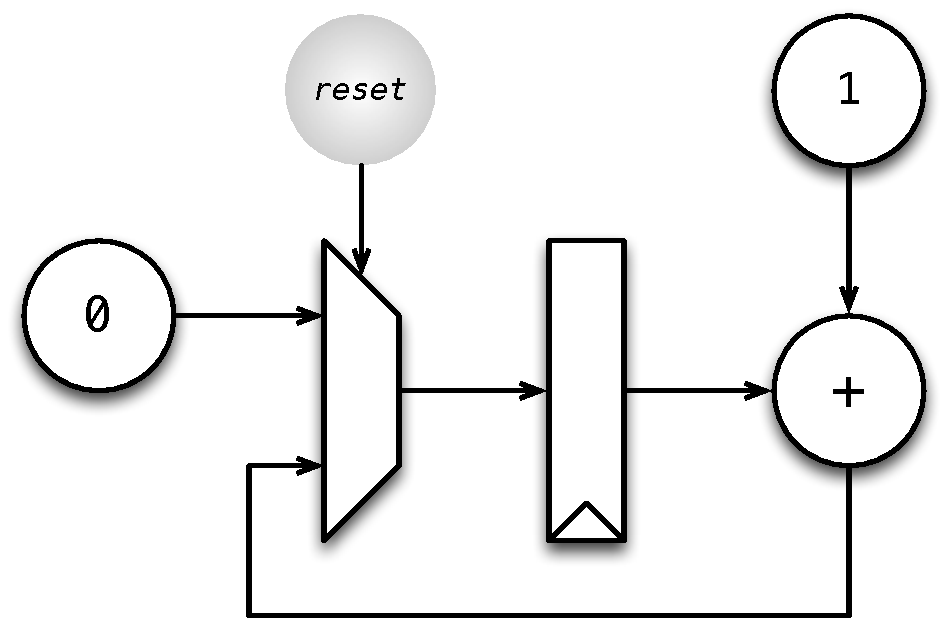
\includegraphics[width=0.9\textwidth]{figs/simple-counter.pdf}
\end{center}
\end{columns}
\begin{itemize}
\item every construct actually creates a concrete circuit
\item know cost of everything
\item layered and can choose level of abstraction
\end{itemize}
\end{frame}

\begin{frame}[fragile]{Hosting Language Ingredients}
Crucial
\begin{itemize}
\item Type Inference
\item Infix Operator Overloading
\item Lightweight Closures
\item Dynamic Scoping
\item Introspection or Simple Macros
\item Functional Programming
\end{itemize}
\vspace{0.5cm}
Even Better with
\begin{itemize}
\item Object Orientation
\item Powerful Macros
\end{itemize}
\end{frame}

\begin{frame}[fragile]{Synthesizable By Construction}
Well formed Chisel graphs are synthesizable.
\begin{columns}
\column{0.6\textwidth}
\begin{itemize}
\item Use small number of basic nodes
\begin{itemize}
\item simple semantics
\item easy to synthesize
\end{itemize}
\item During construction check that
\begin{itemize}
\item types, directions and widths match
\item there are no combinational loops
\end{itemize}
\end{itemize}
\column{0.3\textwidth}
\begin{center}
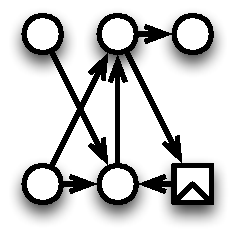
\includegraphics[width=0.9\textwidth]{figs/synthesizable.pdf}
\end{center}
\end{columns}
\vspace{1cm}
\begin{itemize}
\item {\color{red}If it passes these checks then it's synthesizable}
\end{itemize}
\end{frame}

\begin{frame}[fragile]{Hardware Language Approaches}
% \begin{columns}
% \column{0.45\textwidth}
\begin{itemize}
\item {\color{magenta}behavioral} -- high level language compiled to verilog
\begin{itemize}
\item examples: C, Lime, CHP, Esterel, BlueSpec
\end{itemize}
\item {\color{orange}simulation} -- simulation language with synthesizable subset
\begin{itemize}
\item examples: Verilog, System Verilog, SystemC, myHDL
\end{itemize}
\item {\color{green}construction} -- programmatically construct circuits
\begin{itemize}
\item examples: Chisel, Lava
\end{itemize}
\end{itemize}
% \column{0.45\textwidth}
% \begin{center}
% 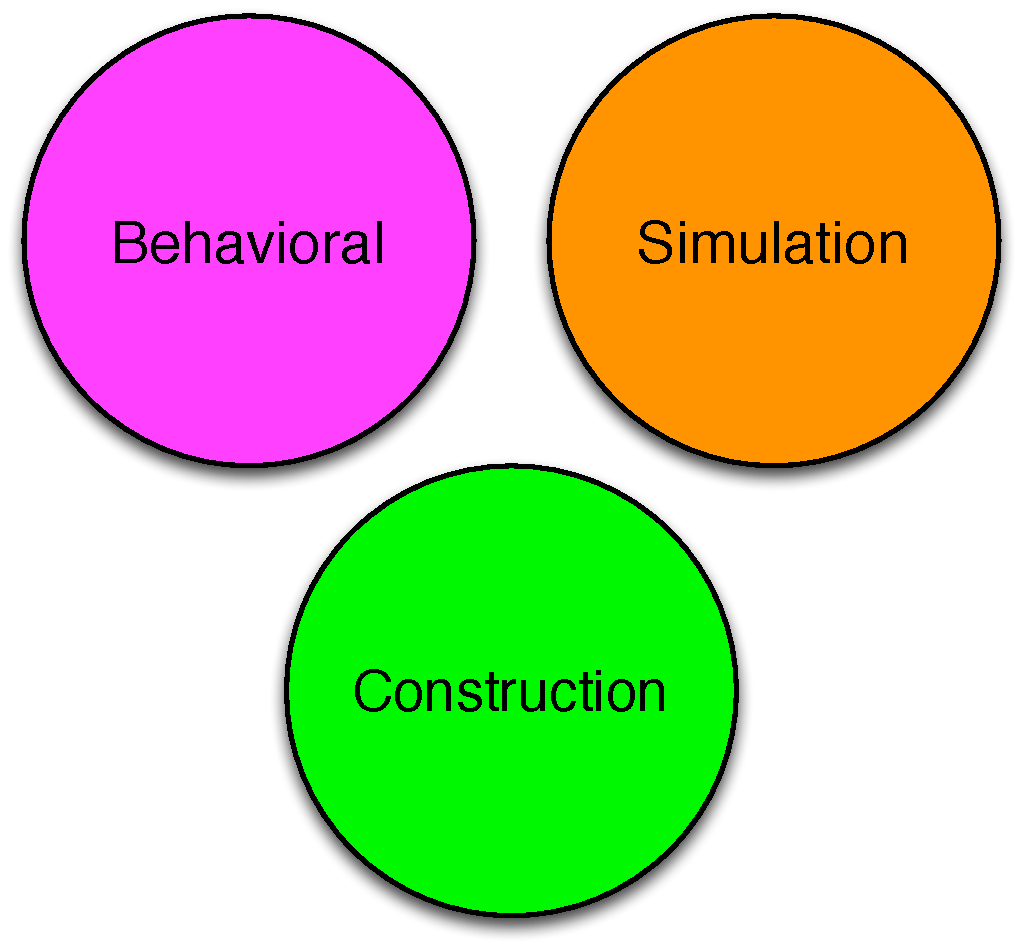
\includegraphics[width=1.0\textwidth]{figs/hdls.pdf} 
% \end{center}
% \end{columns}
\end{frame}

\begin{frame}[fragile]{Hardware Language Comparisons}
\begin{small}
\begin{center}
\begin{tabular}{|r|c|c|c|}
\hline
{\bf name} & {\bf example} & {\bf pros} & {\bf cons} \\ 
\hline
{\color{magenta}behavioral} & C-to-gates & high level & unpredictable \\
 &  &  & QoR \\
\hline
{\color{orange}simulation} & Verilog & flexible & synthesizable? + \\
 &  &  & low abstraction \\
\hline
{\color{green}construction} & Chisel & metaprogramming + & two levels + \\
 &  & predictable QoR + & blemishes \\
 &  &  synthesizable QoR &  \\
\hline
\end{tabular}
\end{center}
\end{small}

\begin{columns}
\column{0.4\textwidth}
\begin{center}
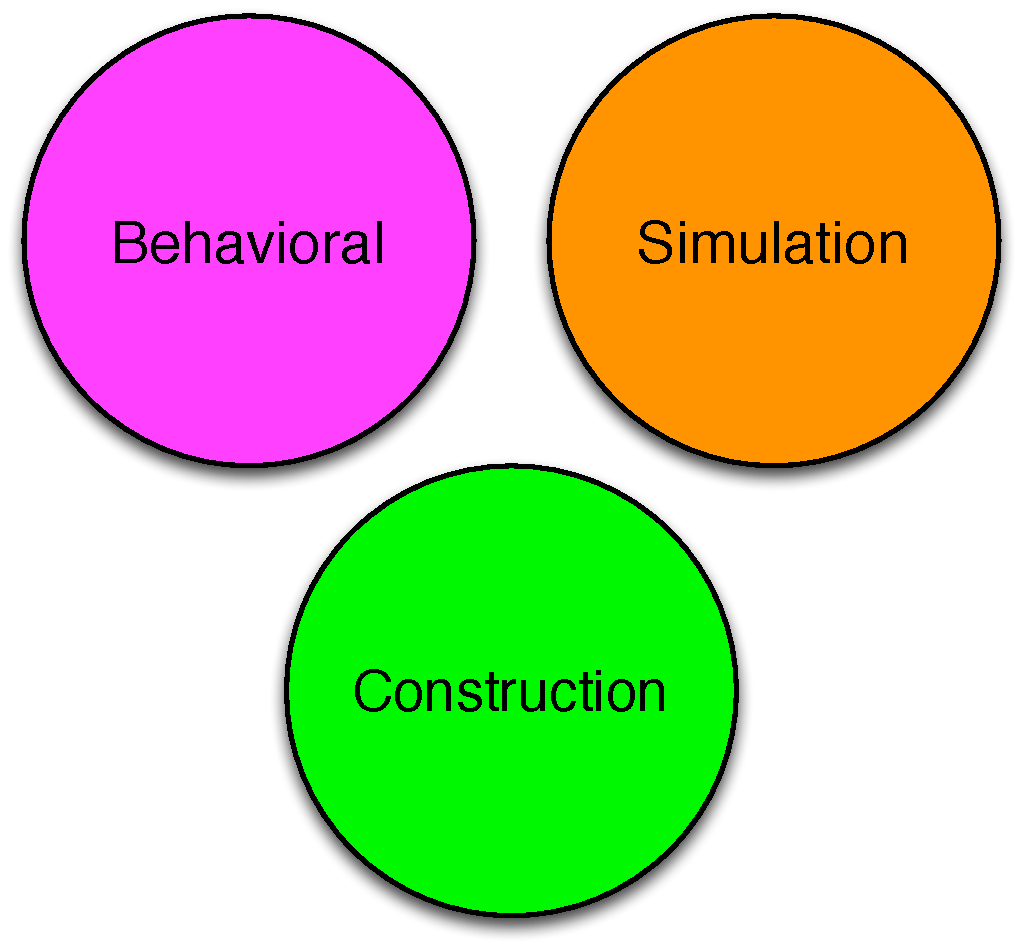
\includegraphics[width=0.8\textwidth]{figs/hdls.pdf} 
\end{center}
\column{0.5\textwidth}
Chisel
\begin{itemize}
\item is {\bf not} Scala to Verilog
\item produces circuits that are synthesizable by construction
\item permits simulation by driving synthesized design
\end{itemize}
\end{columns}
\end{frame}


\setbeamercolor{frametitle}{bg=\frametitleproblemcolor}
\begin{frame}[fragile]{Mul Lookup Table Problem -- \tt Mul.scala}
\begin{itemize}
\item write 16x16 multiplication table using \code{Vec}
\end{itemize}
\begin{scala}
class Mul extends Module {
  val io = new Bundle {
    val x   = UInt(INPUT, 4)
    val y   = UInt(INPUT, 4)
    val z   = UInt(OUTPUT, 8)
  }
  val muls = new ArrayBuffer[UInt]()

  // flush this out ...

  io.z := UInt(0)
}
\end{scala}

hint:
\begin{scala}
val tab = Vec(muls)
io.z := tab(Cat(io.x, io.y))
\end{scala}

\end{frame}
\setbeamercolor{frametitle}{bg=\frametitledefaultcolor}

\begin{frame}[fragile]
\frametitle{Valid Wrapper}

\begin{columns}

\column{0.65\textwidth}

\begin{footnotesize}
\begin{scala}
class Valid[T <: Data](dtype: T) extends Bundle {
  val data  = dtype.clone.asOutput
  val valid = Bool(OUTPUT)
  override def clone = new Valid(dtype)
}

class GCD extends Module {
  val io = new Bundle {
    val a   = UInt(INPUT, 16)
    val b   = UInt(INPUT, 16)
    val out = new Valid(UInt(OUTPUT, 16))
  } }
  ...
  io.out.data  := x
  io.out.valid := y === UInt(0)
}

\end{scala}
\end{footnotesize}

\column{0.3\textwidth}

\begin{center}
\includegraphics[width=0.9\textwidth]{../talks/retreat-1/figs/valid.pdf} 
\end{center}

\end{columns}
\note{now gcd had a valid signal on its output.  \\[1cm]
we can generalize this idea by defining a wrapper class that bundles a valid with a data signal. \\[1cm]
now we can rewrite GCD using an interface using this valid wrapper for its output. }

\end{frame}

\begin{frame}[fragile]
\frametitle{Function Filters}

\begin{footnotesize}
\begin{scala}
abstract class Filter[T <: Data](dtype: T) extends Module {
  val io = new Bundle {
    val in  = Valid(dtype).asInput
    val out = Valid(dtype).asOutput
} }

class FunctionFilter[T <: Data](dtype: T, f: T => T) extends Filter(dtype) {
  io.out.valid := io.in.valid
  io.out.bits  := f(io.in)
}
\end{scala}
\end{footnotesize}

\begin{center}
\includegraphics[height=0.4\textheight]{../talks/sketching13/figs/function-filter.pdf} 
\end{center}

\note{suppose we want to write hardware filters. \\[1cm]
one way to create a reusable filter would be \\[1cm]
to create a filter class that takes a function as argument that definines its filter operation.}

\end{frame}

\begin{frame}[fragile]
\frametitle{Clipping Filter}

\begin{footnotesize}
\begin{scala}
def clippingFilter[T <: Bits](limit: Int, dtype: T) = 
  new FunctionFilter(dtype, x => min(limit, max(-limit, x)))
\end{scala}
\end{footnotesize}

\begin{center}
\includegraphics[height=0.4\textheight]{../talks/retreat-1/figs/clipping-filter.pdf} 
\end{center}
\note{using this reusable substrate then it is easy to create an instance of a filter.}
\end{frame}


\begin{frame}[fragile]
\frametitle{Shifting Filter}

\begin{footnotesize}
\begin{scala}
def shiftingFilter[T <: Bits](shift: Int, dtype: T) = 
  new FunctionFilter(dtype, x => x >> shift)
\end{scala}
\end{footnotesize}

\begin{center}
\includegraphics[height=0.4\textheight]{../talks/retreat-1/figs/shifting-filter.pdf} 
\end{center}
\note{and reuse it for shift filter}
\end{frame}

\begin{frame}[fragile]{Testing Decoupled Circuits}

\begin{itemize}
\item using ovars for outputs
\item need to check outputs directly using \verb+litValue+
\end{itemize}
\begin{scala}
class GCDTests(c: GCD) extends Tester(c) {
  val (a, b, z) = (64, 48, 16)
  do {
    poke(c.io.a, a)
    poke(c.io.b, b)
    step(1)
  } while (t <= 1 || peek(c.io.v) == 0)
  expect(c.io.z, z)
}
\end{scala}

\end{frame}

\begin{frame}[fragile]
\frametitle{Chained Filter}

\begin{footnotesize}
\begin{scala}
class ChainedFilter[T <: Num](dtype: T) extends Filter(dtype) = {
  val shift   = Module(new ShiftFilter(2, dtype))
  val clipper = Module(new ClippingFilter(1 << 7, dtype))
  io.in          <> shift.io.in
  shift.io.out   <> clipper.io.in
  clipper.io.out <> io.out
}
\end{scala}
% \begin{scala}
% class ChainedFilter[T <: Num](dtype: T) extends Filter(dtype) = {
%   val fir     = new TstFIR(dtype)
%   val shift   = new ShiftFilter(2, dtype)
%   val clipper = new ClippingFilter(1 << 7, dtype)
%   io.in          <> fir.io.in
%   fir.io.out     <> shift.io.in
%   shift.io.out   <> clipper.io.in
%   clipper.io.out <> io.out
% }
% \end{scala}
\end{footnotesize}

\begin{center}
\includegraphics[height=0.4\textheight]{../talks/sketching13/figs/chained-filter2.pdf} 
\end{center}
\note{and chain together...}
\end{frame}

\begin{frame}[fragile]{Predicate Filter}
\begin{scala}
class PredicateFilter[T <: Data](dtype: T, f: T => Bool) 
    extends Filter(dtype) {
  io.out.valid := io.in.valid && f(io.in.bits)
  io.out.bits  := io.in.bits
}
\end{scala}

\begin{center}
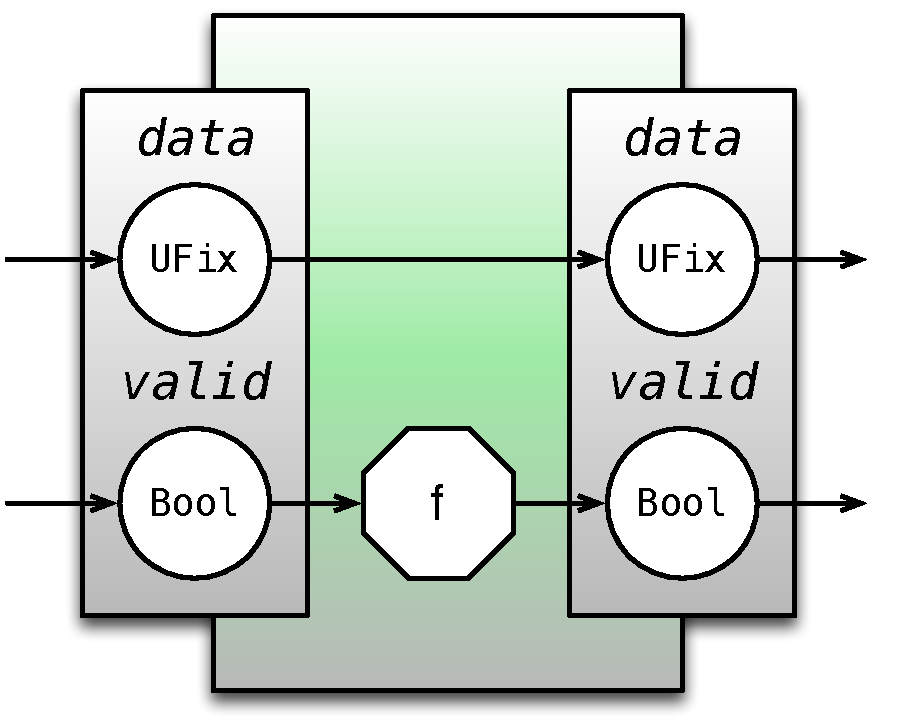
\includegraphics[height=0.4\textheight]{figs/predicate-filter.pdf} 
\end{center}
\end{frame}

\setbeamercolor{frametitle}{bg=\frametitleproblemcolor}
\begin{frame}[fragile]{Predicate Filtering -- \tt SingleEvenFilter.scala}
\begin{itemize}
\item write filter that lets only even single digit numbers through
\end{itemize}
\begin{scala}
object SingleFilter {
  def apply[T <: UInt](dtype: T) = // FILL IN FUNCTION BELOW
    Module(new PredicateFilter(dtype, (x: T) => Bool(false)))
}

object EvenFilter {
  def apply[T <: UInt](dtype: T) = // FILL IN FUNCTION BELOW
    Module(new PredicateFilter(dtype, (x: T) => Bool(false)))
}

class SingleEvenFilter[T <: UInt](dtype: T) extends Filter(dtype) {
  // FILL IN CONSTRUCTION AND WIRING
  io.out := UInt(0)
}
\end{scala}
\end{frame}
\setbeamercolor{frametitle}{bg=\frametitledefaultcolor}

\begin{frame}[fragile, shrink]
\frametitle{Functional Composition}

% \begin{itemize}
% \item natural
% \item reusable
% \item composable
% \end{itemize}
% \vskip1cm

\begin{Large}
\begin{columns}

\column{0.45\textwidth}
\verb+Map(ins, x => x * y)+ \\
\begin{center}
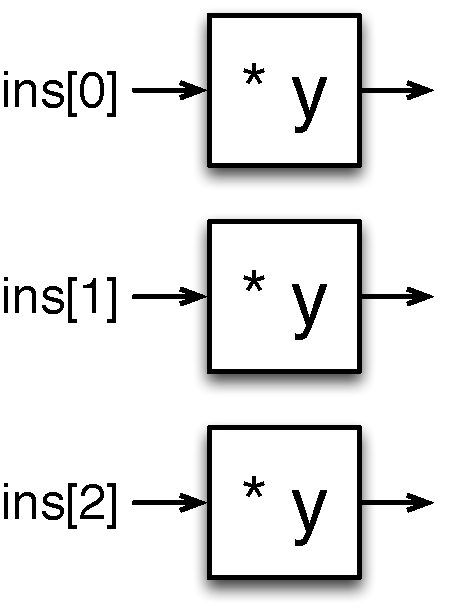
\includegraphics[height=0.6\textheight]{../bootcamp/figs/map.pdf} \\[2cm]
\end{center}

\column{0.45\textwidth}
\vskip2mm
\verb+Chain(n, in, x => f(x))+ \\
\begin{center}
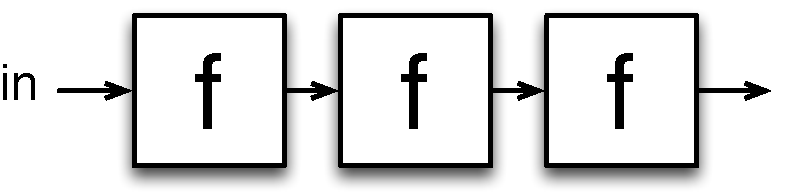
\includegraphics[width=0.9\textwidth]{../bootcamp/figs/chain.pdf} \\
\end{center}

\verb+Reduce(ins, Max)+ \\
\begin{center}
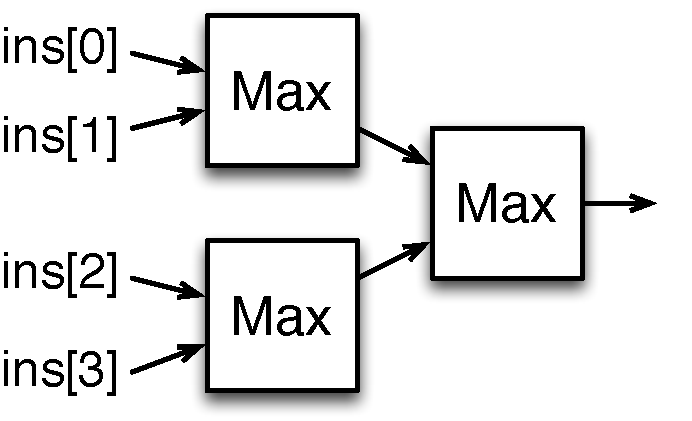
\includegraphics[width=0.9\textwidth]{../bootcamp/figs/reduce.pdf} \\
\end{center}

\end{columns}

\end{Large}
\note{the previous example showed a simple use of functional programming. \\[1cm]
Scala provides strong support for functional programming and
it turns out that functional programming is a powerful way to define hardware. \\[1cm]
for example, you can create a parallel set of blocks using map and reduce to creation reduction trees and chain to create a pipeline.}
\end{frame}

\begin{frame}[fragile]{Flo Map / Reduce Generator}

{\lstset{basicstyle={\scriptsize\ttfamily}}
\begin{scala}
object FloDelays {
  def apply(x: Flo, n: Int): List[Flo] = 
    if (n <= 1) List(x) else x :: FloDelays(RegNext(x), n-1)
}
object FloFIR {
  def apply(ws: Seq[Flo], x: T): T = 
    (ws, FloDelays(x, ws.length)).zipped.map( _ * _ ).reduce( _ + _ )
}
class FIR extends Module {
  val io = new Bundle { val x = Flo(INPUT); val z = Flo(OUTPUT) }
  val ws = Array(Flo(0.25), Flo(0.75))
  io.z  := FloFIR(ws, io.x)
}
\end{scala}
}
\begin{center}
\includegraphics[height=0.35\textheight]{../cs294-88/lectures/advanced-chisel/figs/inner-product-fir.png} 
\end{center}
\note{as an advanced example, consider writing an FIR filter which is defined by the equation below. \\[1cm]
essentially it's a sum of products of coefficients and delayed versions of input.\\[1cm]
we can write this quite simply using map and reduce as above.}
\end{frame}

\begin{frame}[fragile]{Generic Map / Reduce Generator}

{\lstset{basicstyle={\scriptsize\ttfamily}}
\begin{scala}
object Delays {
  def apply[U <: Data](x: U, n: Int): List[U] = 
    if (n <= 1) List(x) else x :: Delays(RegNext(x), n-1)
}
object GenFIR {
  def apply[T <: Data with Num[T]](ws: Seq[T], x: T): T = 
    (ws, Delays(x, ws.length)).zipped.map( _ * _ ).reduce( _ + _ )
}
class FIR extends Module {
  val io = new Bundle { val x = Flo(INPUT); val z = Flo(OUTPUT) }
  val ws = Array(Flo(0.25), Flo(0.75))
  io.z  := GenFIR(ws, io.x)
}
\end{scala}
}
\begin{center}
\includegraphics[height=0.35\textheight]{../cs294-88/lectures/advanced-chisel/figs/inner-product-fir.png} 
\end{center}
\note{as an advanced example, consider writing an FIR filter which is defined by the equation below. \\[1cm]
essentially it's a sum of products of coefficients and delayed versions of input.\\[1cm]
we can write this quite simply using map and reduce as above.}
\end{frame}

\begin{frame}[fragile]{Chisel Standard Library -- \tt ChiselUtil.scala}
\begin{center}
\begin{tabular}{rl}
{\bf Bits Properities} & \code{log2Up}, \code{log2Down}, \code{isPow2}, \code{PopCount}\\
{\bf Numeric Utilities} & \code{LFSR16}, \code{Reverse}, \code{FillInterleaved} \\
{\bf Stateful Functions} & \code{ShiftRegister}, \code{Counter} \\
{\bf Priority Encoding Functions} & \code{UIntToOH}, \code{OHToUInt}, \code{Mux1H} \\
{\bf Priority Encoders} & \code{PriorityEncoder}, \code{PriorityEncoderOH}  \\
{\bf Vec Construction} & \code{Vec.fill}, \code{Vec.tabulate} \\
{\bf Vec Functional} & \code{forall}, \code{exists}, \code{contains}, ... \\
{\bf Queues and Pipes} & \code{Decoupled}, \code{Queue}, \code{Valid}, \code{Pipe} \\
{\bf Arbiters} & \code{ArbiterIO}, \code{Arbiter}, \code{RRArbiter} \\
\end{tabular}
\end{center}
\end{frame}

\begin{frame}[fragile]
\frametitle{Queues}
\begin{itemize}
\item Required parameter \verb+entries+ controls depth
\item The width is determined from the inputs.
\end{itemize}
\begin{scala}
class QueueIO[T <: Data](type: T, entries: Int) extends Bundle {
  val enq   = Decoupled(data.clone).flip
  val deq   = Decoupled(data.clone)
  val count = UFix(OUTPUT, log2Up(entries+1))
}

class Queue[T <: Data]
    (type: T, entries: Int, 
     pipe: Boolean = false,
     flow: Boolean = false)
    extends Module  
\end{scala}
\begin{scala}
val q = new Queue(UInt(), 16)
q.io.enq <> producer.io.out
consumer.io.in <> q.io.deq
\end{scala}
\end{frame}

\begin{frame}[fragile]{Multiple Clock Domains}
Clocks are first class and take a name argument:
\begin{scala}
class Clock (val name: String) extends Node { 
}
\end{scala}
\noindent
and when constructed define a clock at top-level with the given name:
\begin{scala}
val clkA = new Clock("A")
\end{scala}

There is a builtin implicit clock that state elements use by default:
\begin{scala}
class Module {
  def clock(): Clock    
  def reset(): Bool
  ...
}
\end{scala}
 
% Clocks can be defined from other clocks:
% \begin{scala} 
% val clock2 = clock1 * 2 
% val clock3 = clock1 / 2 
% \end{scala}

\end{frame}

\begin{frame}[fragile]{Specifying a Clock Domain}
The clock for state elements and modules can be specified:
\begin{scala} 
Reg(... explClock: Clock = clock()) 
Mem(... explClock: Clock = clock()) 
Module(... explClock: Clock = clock())
\end{scala}

For example, a register can be created in a different clock domain as follows:
\begin{scala} 
val reg = Reg(UInt(), explClock = clock2)
\end{scala}

\end{frame}
 
\begin{frame}[fragile]{Crossing Clock Domains}
The most general technique to send data between domains is using an
asynchronous queue or fifo:

\begin{scala} 
class AsyncFifo[T <: Data]
    (dataType: T, entries: Int, enq_clk: Clock, deq_clock: Clock) extends Module
\end{scala}
 
Using these fifos, we can then move a signalA from clock domains clockA to signalB in clockB:

\begin{scala} 
val queue = new AsyncFifo(Uint(width = 32), 2, clockA, clockB) 
fifo.enq.bits := signalA 
signalB       := fifo.deq.bits 
fifo.valid    := condA 
fifo.ready    := condB 
...
\end{scala}

\end{frame}

\begin{frame}[fragile]{Multiple Clocks -- \tt MultipleClockDomains.scala}
\begin{scala}
class MultiClockDomain extends Module {
  val io = new Bundle {
    val start = Bool(INPUT)
    val sum = Decoupled(UInt(OUTPUT))
  }
  val fastClock = new Clock()
  val slowClock = new Clock()
  ...
}

class MultiClockDomainTests(c: MultiClockDomain) 
    extends Tester(c, Array(c.io)) {
  val clocks = new HashMap[Clock, Int]
  clocks(Module.implicitClock) = 2
  clocks(c.fastClock) = 4
  clocks(c.slowClock) = 6
  setClocks(clocks)
  ...
}
\end{scala}
\end{frame}

\begin{frame}[fragile]{Creating Your Own Project}
directory structure
\begin{bash}
Hello/
  build.sbt   # scala configuration file
  Hello.scala # your source file
\end{bash}

\end{frame}

\begin{frame}[fragile]{Writing Your Source File}

{\lstset{basicstyle={\scriptsize\ttfamily}}
\begin{scala}
package Hello
import Chisel._

class Hello extends Module {
  val io = new Bundle { 
    val out = UInt(OUTPUT, 8) }
  io.out := UInt(33)
}

class HelloTests(c: Hello) extends Tester(c) {
  step(1)
  expect(c.io.out, 33)
}

object Hello {
  def main(args: Array[String]): Unit = {
    val args = Array("--backend", "c", "--genHarness", "--compile", "--test")
    chiselMainTest(args, () => Module(new Hello())) {
      c => new HelloTests(c) }
} }
\end{scala}
}

\end{frame}

\begin{frame}[fragile]{Setting Up Your SBT Configuration File}
\begin{scala}
scalaVersion := "2.10.2"

addSbtPlugin("com.github.scct" % "sbt-scct" % "0.2")

libraryDependencies += 
  "edu.berkeley.cs" %% "chisel" % "latest.release"
\end{scala}
\end{frame}

\begin{frame}[fragile]{Compiling and Running}
Producing C++
\begin{bash}
sbt run "--backend c"
\end{bash}

Producing Verilog
\begin{bash}
sbt run "--backend v"
\end{bash}

Running the Chisel Tests
\begin{bash}
sbt run "--backend c --compile --test --genHarness"
\end{bash}

\end{frame}

\begin{frame}[fragile]{chiselMain(Test) Command Line Arguments}
\begin{scala}
sbt 
sbt> compile         // compiles Chisel Scala code
sbt> run             // compile and run Chisel Scala Code
sbt> run --backend c // produces C++ files
sbt> exit
\end{scala}

with a complete set of command line arguments being:\\[2mm]

\begin{tabular}{lll}
\verb+--backend v+ & generate verilog \\
\verb+--backend c+ & generate C++ (default)\\
\verb+--vcd+ & enable vcd dumping \\
\verb+--targetDir+ & target pathname prefix \\
\verb+--genHarness+ & generate harness file for C++ \\
\verb+--debug+ & put all wires in C++ class file \\
\verb+--compile+ & compiles generated C++ \\
\verb+--test+ & runs tests using C++ app \\
\end{tabular}
\end{frame}

\setbeamercolor{frametitle}{bg=\frametitleproblemcolor}
\begin{frame}[fragile]{Make Your Own Project}
set hello project up
\begin{bash}
cd ~
mkdir hello
cp -r ~/chisel-tutorial/hello/* hello
cd hello
sbt run
\end{bash}
make a change
\begin{itemize}
\item make output a function of an new input 
\end{itemize}
\end{frame}
\setbeamercolor{frametitle}{bg=\frametitledefaultcolor}

\begin{frame}{Chisel Workflow}
\begin{center}
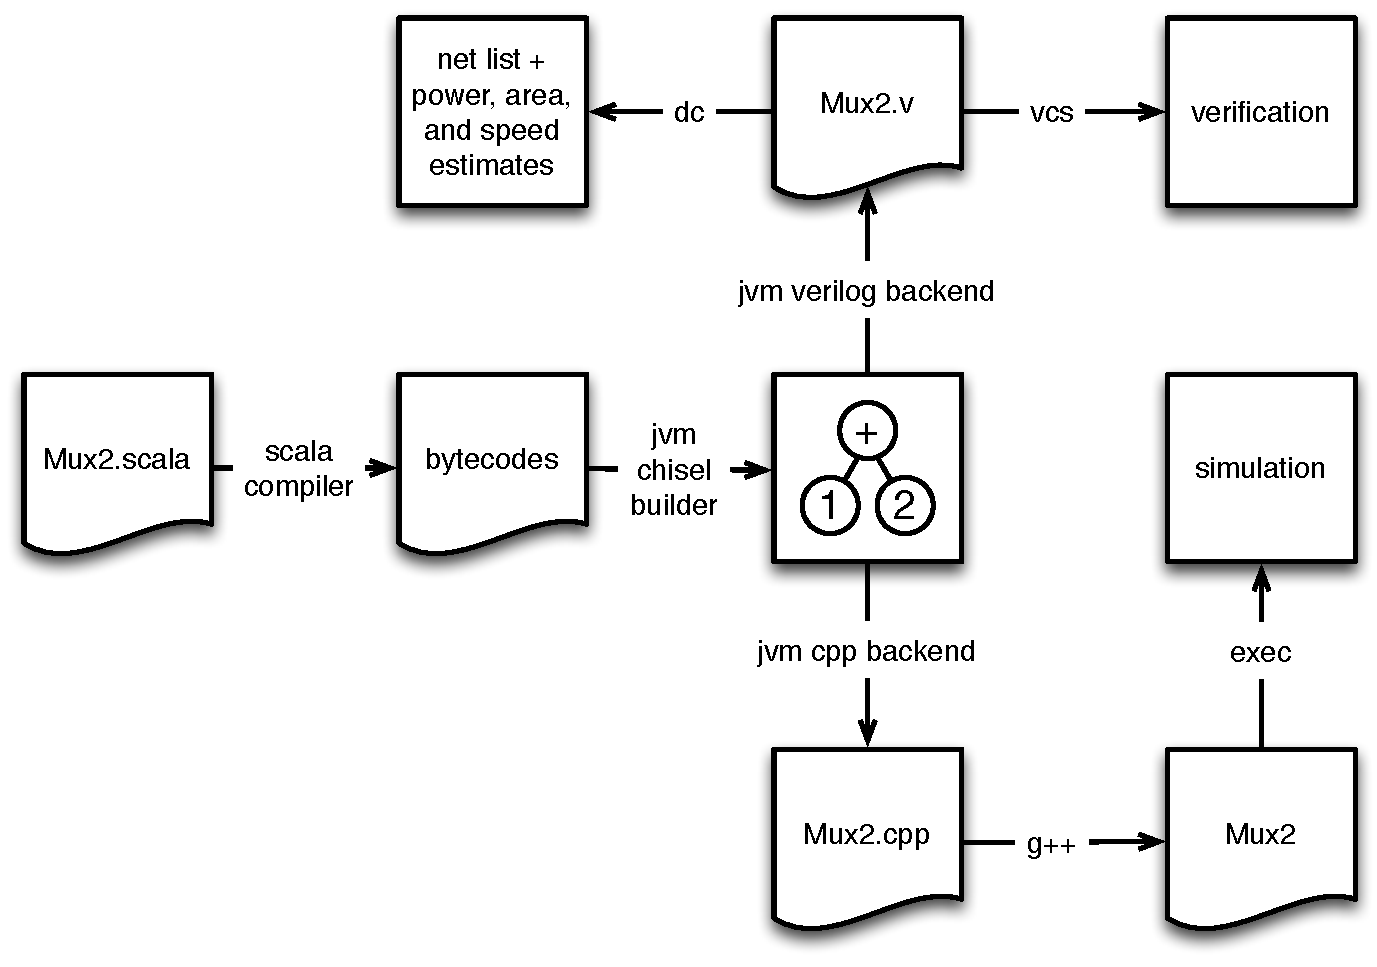
\includegraphics[height=0.9\textheight]{../bootcamp/figs/chisel-workflow.pdf}
\end{center}
\end{frame}

\begin{frame}[fragile]{printf / sprintf}
\begin{itemize}
\item during simulation
\begin{itemize}
\item \verb+printf+ prings the formatted string to the console on rising clock edges
\item \verb+sprintf+ returns the formatted string as a bit vector
\end{itemize}
\item format specifiers are
\begin{itemize}
\item \verb+%b+ -- binary number
\item \verb+%d+ -- decimal number
\item \verb+%x+ -- hexidecimal number
\item \verb+%e+ -- floating point number in scientific notation
\item \verb+%s+ -- string consisting of a sequence of 8-bit extended ASCII chars
\item \verb+%%+ -- specifies a literal %.
\end{itemize}
\end{itemize}
the following prints the line \verb+"0x4142 16706 AB"+ on cycles when \verb+c+ is true:
\begin{scala}
val x = Bits(0x4142)
val s1 = sprintf("%x %s", x, x);
when (c) { printf("%d %s\n", x, s1); }
\end{scala}
\end{frame}

\begin{frame}[fragile]{assert}
\begin{itemize}
\item simulation time assertions are provided by \verb+assert+ construct
\item if assert arguments false on rising edge then 
\begin{itemize}
\item an error is printed and 
\item simulation terminates
\end{itemize}
\end{itemize}
the following will terminate after 10 clock cycles:
\begin{scala}
val x = Reg(init = UInt(0, 4))
x := x + UInt(1)
assert(x < UInt(10))
\end{scala}
\end{frame}

\begin{frame}[fragile]{Installation}
\begin{itemize}
\item on mac install:
\begin{itemize}
\item XCODE console tools
\end{itemize}
\item on windows install:
\begin{itemize}
\item cygwin
\end{itemize}
\item everywhere install:
\begin{itemize}
\item git
\item g++ version 4.0 or later
\item java
\end{itemize}
\item everywhere
\begin{itemize}
\item git clone https://github.com/ucb-bar/chisel-tutorial.git
\end{itemize}
\end{itemize}

\end{frame}

\begin{frame}[fragile]{Chisel Resources}
\begin{center}
\url{https://chisel.eecs.berkeley.edu/documentation.html} \\[0.25cm]
\begin{tabular}{rl}
\textbf{getting started} & \code{getting-started.pdf} \\
\textbf{tutorial} & \code{tutorial.pdf} \\
\textbf{manual} & \code{manual.pdf} \\
% \textbf{bootcamp} & \code{bootcamp.pdf} \\
\end{tabular}
\url{https://github.com/ucb-bar/chisel/} \\[0.25cm]
\begin{tabular}{rl}
\textbf{setup} & \code{readme.md} \\
\textbf{utils} & \code{src/main/scala/ChiselUtils.scala} \\[0.5cm]
\end{tabular}
\url{https://chisel.eecs.berkeley.edu/download.html} \\[0.25cm]
\begin{tabular}{rl}
\textbf{sodor} & \url{https://github.com/ucb-bar/riscv-sodor/} \\
% \textbf{virtualbox} & \url{https://chisel.eecs.berkeley.edu/chisel-riscv.box} \\
\end{tabular}
\end{center}
\end{frame}

\begin{frame}{Scala Resources}

\begin{center}

\includegraphics[height=0.4\textheight]{../bootcamp/figs/programming-scala.pdf} \\
\includegraphics[height=0.4\textheight]{../bootcamp/figs/programming-in-scala.pdf}
\end{center}

\end{frame}

\begin{frame}[fragile]{Projects Ideas}
 
\begin{center}
\begin{tabular}{rl}
\textbf{audio processing} & \code{Echo.scala} \\
\textbf{image processing} & \code{Darken.scala} \\
\textbf{risc processor} & \code{Risc.scala} \\
\textbf{game of life} & \code{Life.scala} \\
\textbf{router} & \code{Router.scala} \\
\textbf{map/reduce} & \code{FIR.scala}\\
\textbf{network} & \\
\textbf{decoupled filter} & \\
\textbf{cryptography} & \\
\textbf{serial multiplier} & \\
\textbf{pong} & \\
\end{tabular}
\end{center}

\end{frame}

\begin{frame}[fragile]{Keep in Touch}
\begin{center}
\begin{tabular}{rl}
\textbf{website} & \url{chisel.eecs.berkeley.edu} \\
\textbf{mailing list} & \url{groups.google.com/group/chisel-users} \\
\textbf{github} & \url{https://github.com/ucb-bar/chisel/} \\
\textbf{features + bugs} & \url{https://github.com/ucb-bar/chisel/issues} \\
\textbf{more questions} & \url{stackoverflow.com/quesions/tagged/chisel} \\
\textbf{twitter} & {\tt \#chiselhdl} \\
\textbf{me} & \url{jrb@eecs.berkeley.edu} \\
\end{tabular}
\end{center}
\end{frame}

\begin{frame}{Thanks}
\begin{itemize}
\item \textbf{Arrangements} -- HPCA folks
\item \textbf{USB Sticks} -- Albert Magyar + Jim Lawson
\item \textbf{Bootcamp Materials} -- JB, Vincent Lee, Stephen Twigg, Huy Vo
\item \textbf{Funding} -- Department of Energy, Department of Defense, StarNet, C-Far, LBNL, Intel, Google, LG, Nvidia, Samsung, Oracle, Huawei
\end{itemize}
\end{frame}

\end{document}
